% Chapter Template

\chapter{Visualizaciones} % Main chapter title

\label{VISUALIZACIÓN} % Change X to a consecutive number; for referencing this chapter elsewhere, use \ref{ChapterX}

%----------------------------------------------------------------------------------------
%	SECTION 1
%------------------------5---------------------------------------------------------------

\section{Representaciones clásicas del mutualismo}

Las visualizaciones son una herramienta cada día más importante en el análisis de la información, y en particular en la ciencia de redes. La representación gráfica resulta fundamental en el análisis exploratorio pero también para la síntesis de los resultados. Para redes ecológicas se emplean gráficos de uso común en la representación de redes sociales \cite{freeman2012social}. Quizá porque su tamaño es reducido en comparación con otras aplicaciones, no ha habido apenas desarrollo de herramientas y gráficas específicas para este campo de aplicación \cite{yoon20043d, kazanci2007econet}.

En el análisis del mutualismo se utilizan de forma reiterada dos representaciones: el diagrama bipartito y la matriz de interacción. Ambas  son sencillas y ponen de manifiesto la separación entre clases de especies, pero tienen inconvenientes importantes. 

En el diagrama bipartito se disponen las especies en dos filas paralelas, ya sean horizontales o verticales
y se unen aquellas que interactúan.

\begin{figure}[h!]
\centering
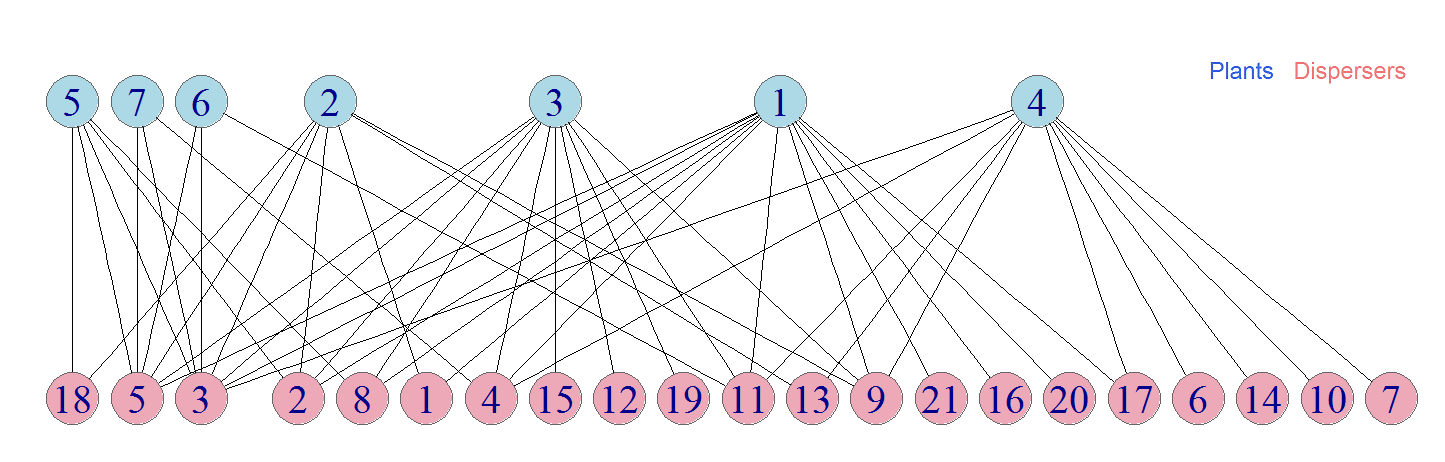
\includegraphics[scale=0.33]{Figures/VIS_bipartito_SD_001.png}
\caption{Diagrama bipartito de una red de dispersores en New Jersey \cite{baird1980selection}.}
\label{fig:VIS_bipartito_SD_001}
\end{figure}

En el ejemplo de la figura \ref{fig:VIS_bipartito_SD_001} la red es de un tamaño reducido, puede distinguirse el núcleo de plantas más conectadas (de la $1$ a la $4$ y los enlaces se ven con claridad. Cuando el número de especies supera unas pocas decenas, la situación cambia de forma radical.

\begin{figure}[h!]
\centering
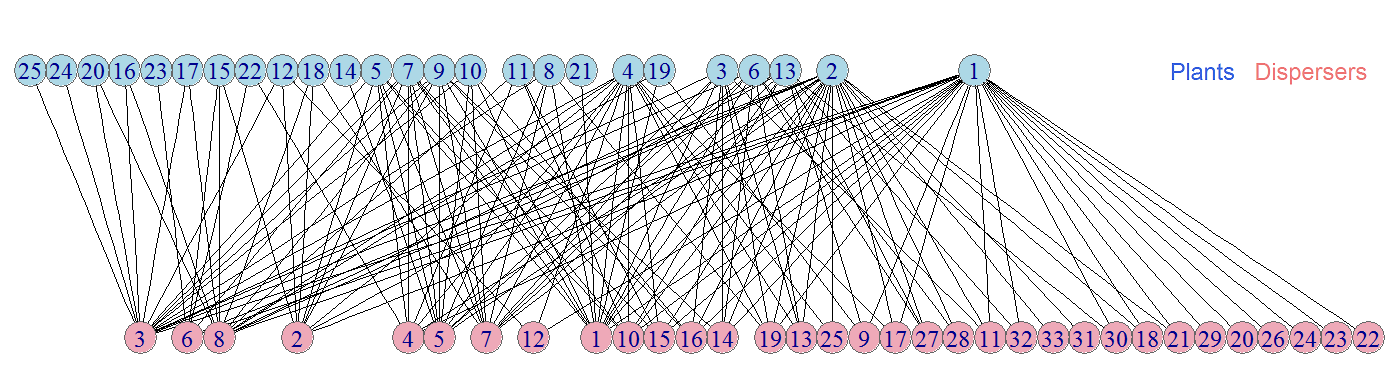
\includegraphics[scale=0.4]{Figures/VIS_bipartito_SD_020.png}
\caption{Red de dispersores en Nava Correhuelas, Sierra de Cazorla, España. Compilada por Pedro Jordano, no publicada.}
\label{fig:VIS_bipartito_SD_020}
\end{figure}

La red de la figura \ref{fig:VIS_bipartito_SD_020} tiene $58$ especies y $150$ enlaces, frente a $28$ especies y $50$ enlaces de la anterior. Es una red de dimensiones moderadas, pero ya es muy complicado seguir los detalles del gráfico. A pesar de ello, algunos autores consiguen resultados excelentes con redes de dimensiones similares a las de este segundo ejemplo, jugando con formas, colores y tamaños \cite{dakos2014critical}. Cuando se llega al centenar de especies, la zona central degenera en una mancha en la que es imposible distinguir los enlaces. Por este motivo, en la literatura sobre mutualismo solo aparecen gráficos de redes pequeñas. 

La matriz de interacción ofrece una visión más rica si los nodos se ordenan de la forma adecuada. Colocando los más conectados en la parte superior izquierda, es fácil localizar el núcleo de especies generalistas. Con redes pequeñas como la del primer ejemplo, el resultado es muy satisfactorio.

\begin{figure}[h!]
\centering
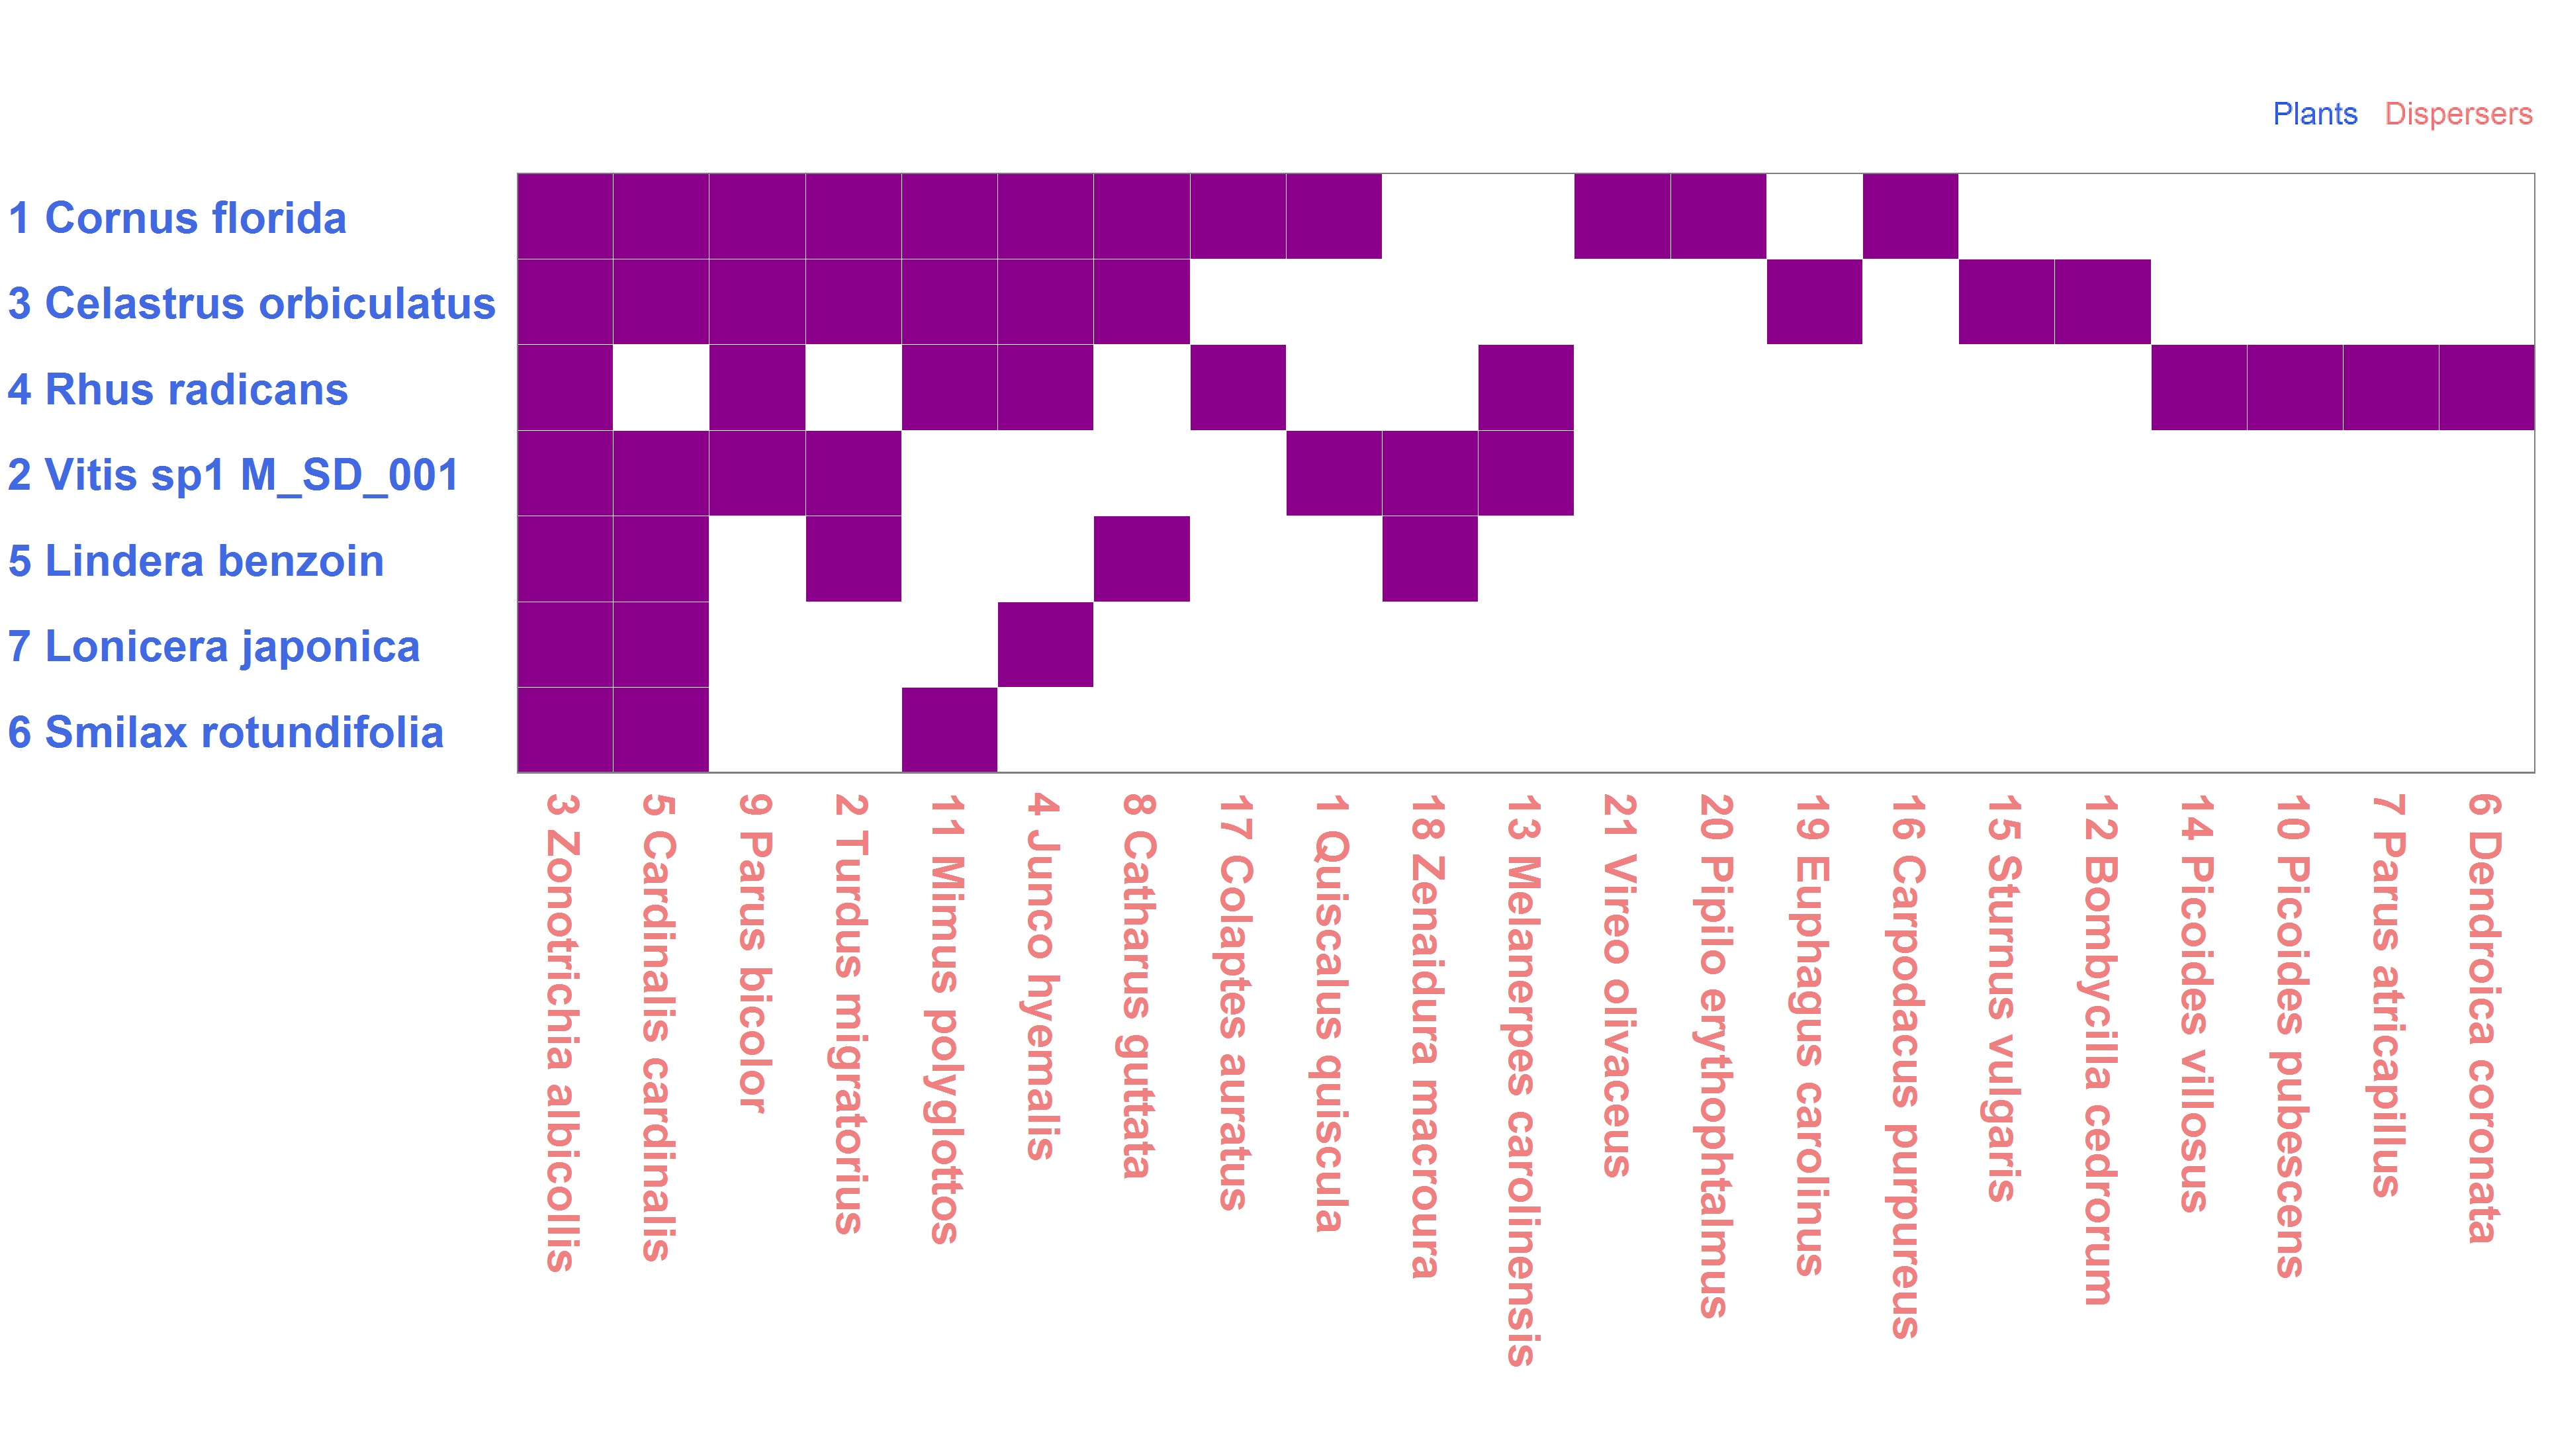
\includegraphics[scale=0.4]{Figures/VIS_matrix_SD_001.png}
\caption{Matriz de interacción de una red de dispersores en New Jersey \cite{baird1980selection}. Las casillas coloreadas indican la existencia de enlace.}
\label{fig:VIS_matrix_SD_001}
\end{figure}

Por el contrario, la matriz de interacción se vuelve también muy confusa para redes grandes, como muestra la figura \ref{fig:VIS_matrix_PL_001}.

\begin{figure}[h!]
\centering
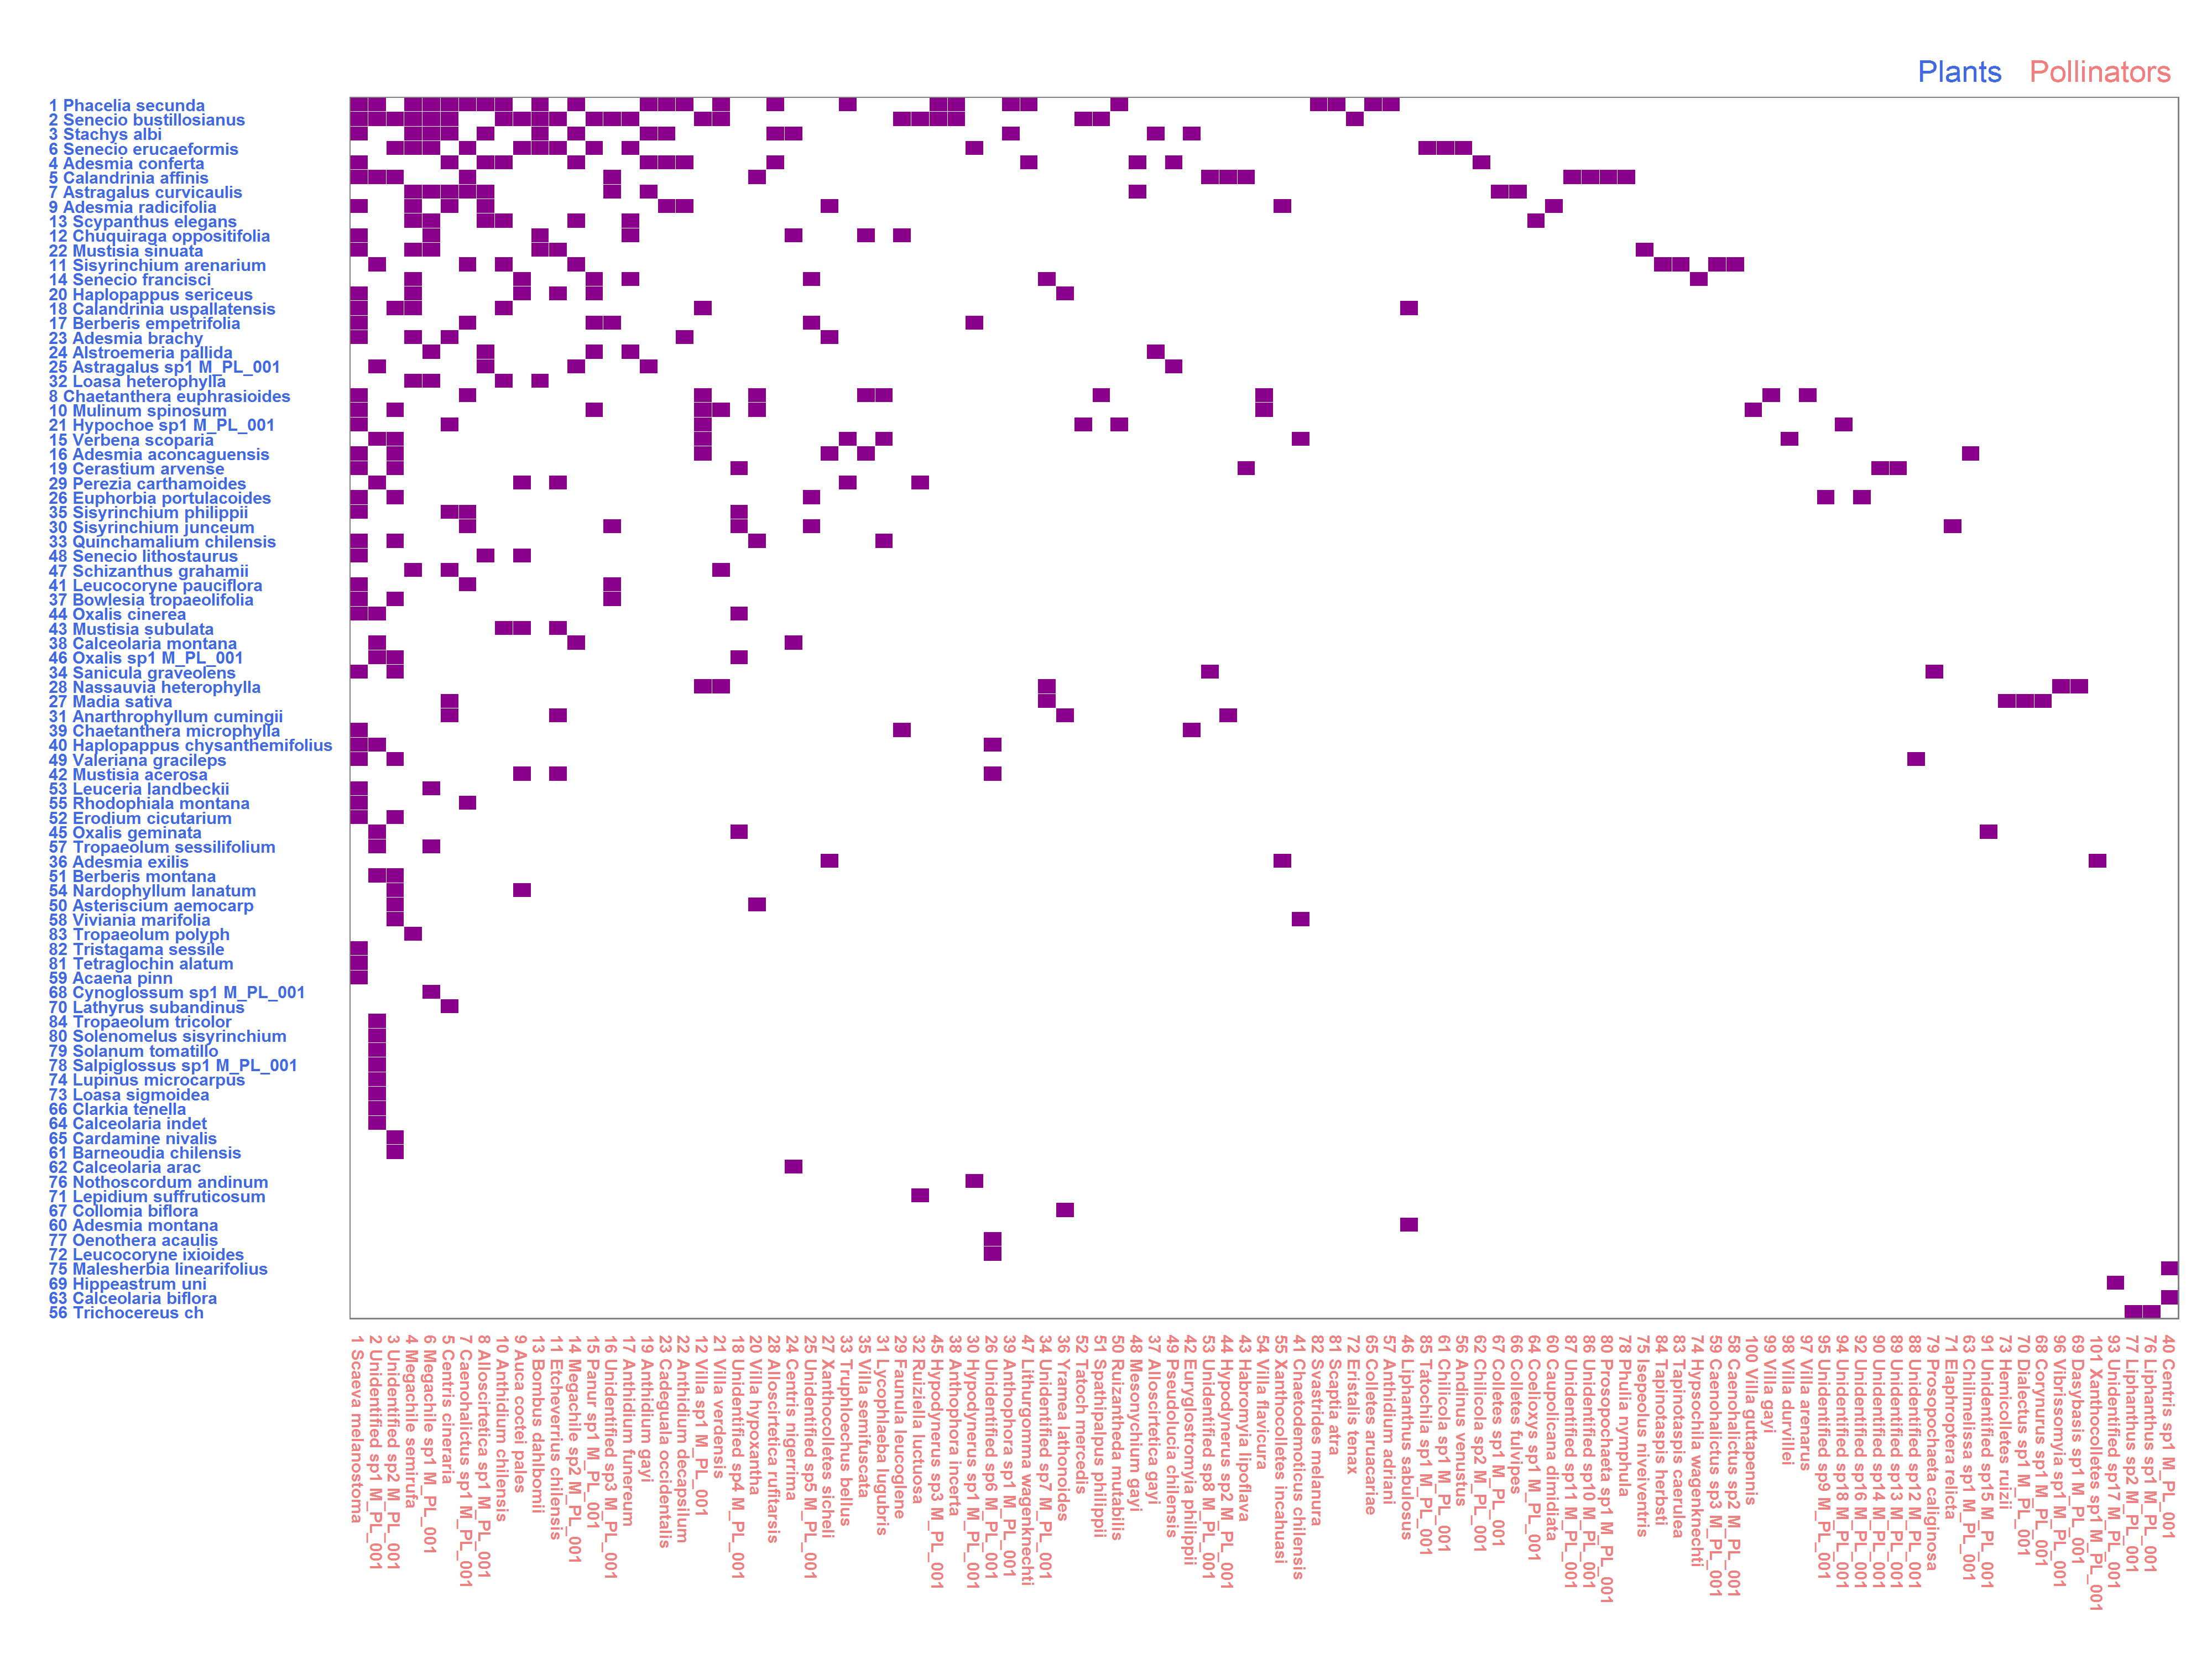
\includegraphics[scale=0.4]{Figures/VIS_matrix_PL_001.png}
\caption{Matriz de interacción de una red de polinizadores en Los Andes, Chile \cite{arroyo1982community}.}
\label{fig:VIS_matrix_PL_001}
\end{figure}


\section{Visualizaciones basadas en \textit{k-magnitudes}}

En este apartado se describen dos nuevos tipos de visualización que se basan en las \textit{k magnitudes} definidas en el capítulo anterior: el diagrama polar y el diagrama zigurat.

\subsection{El diagrama polar}

El diagrama polar se inspira en el \textit{fingerprint plot}, desarrollado por Álvarez-Hamelin \textit{et al} y que se basa en la descomposición \textit{k-core} \cite{alvarez2005k}. Los autores emplearon la técnica para reducir la información y poder visualizar redes muy grandes con índice $k$ máximo del orden de varias decenas. Los nodos se ubican de manera concénrica, a una distancia inversamente proporcional a la \textit{k-shell} a la que pertenecen. No se representan todos los enlaces, solo los más pesados. Una versión más evolucionada no utiliza los nodos sino las \textit{k-shell} que se disponen en espiral \cite{barbera2015critical}.

\begin{figure}[h!]
\centering
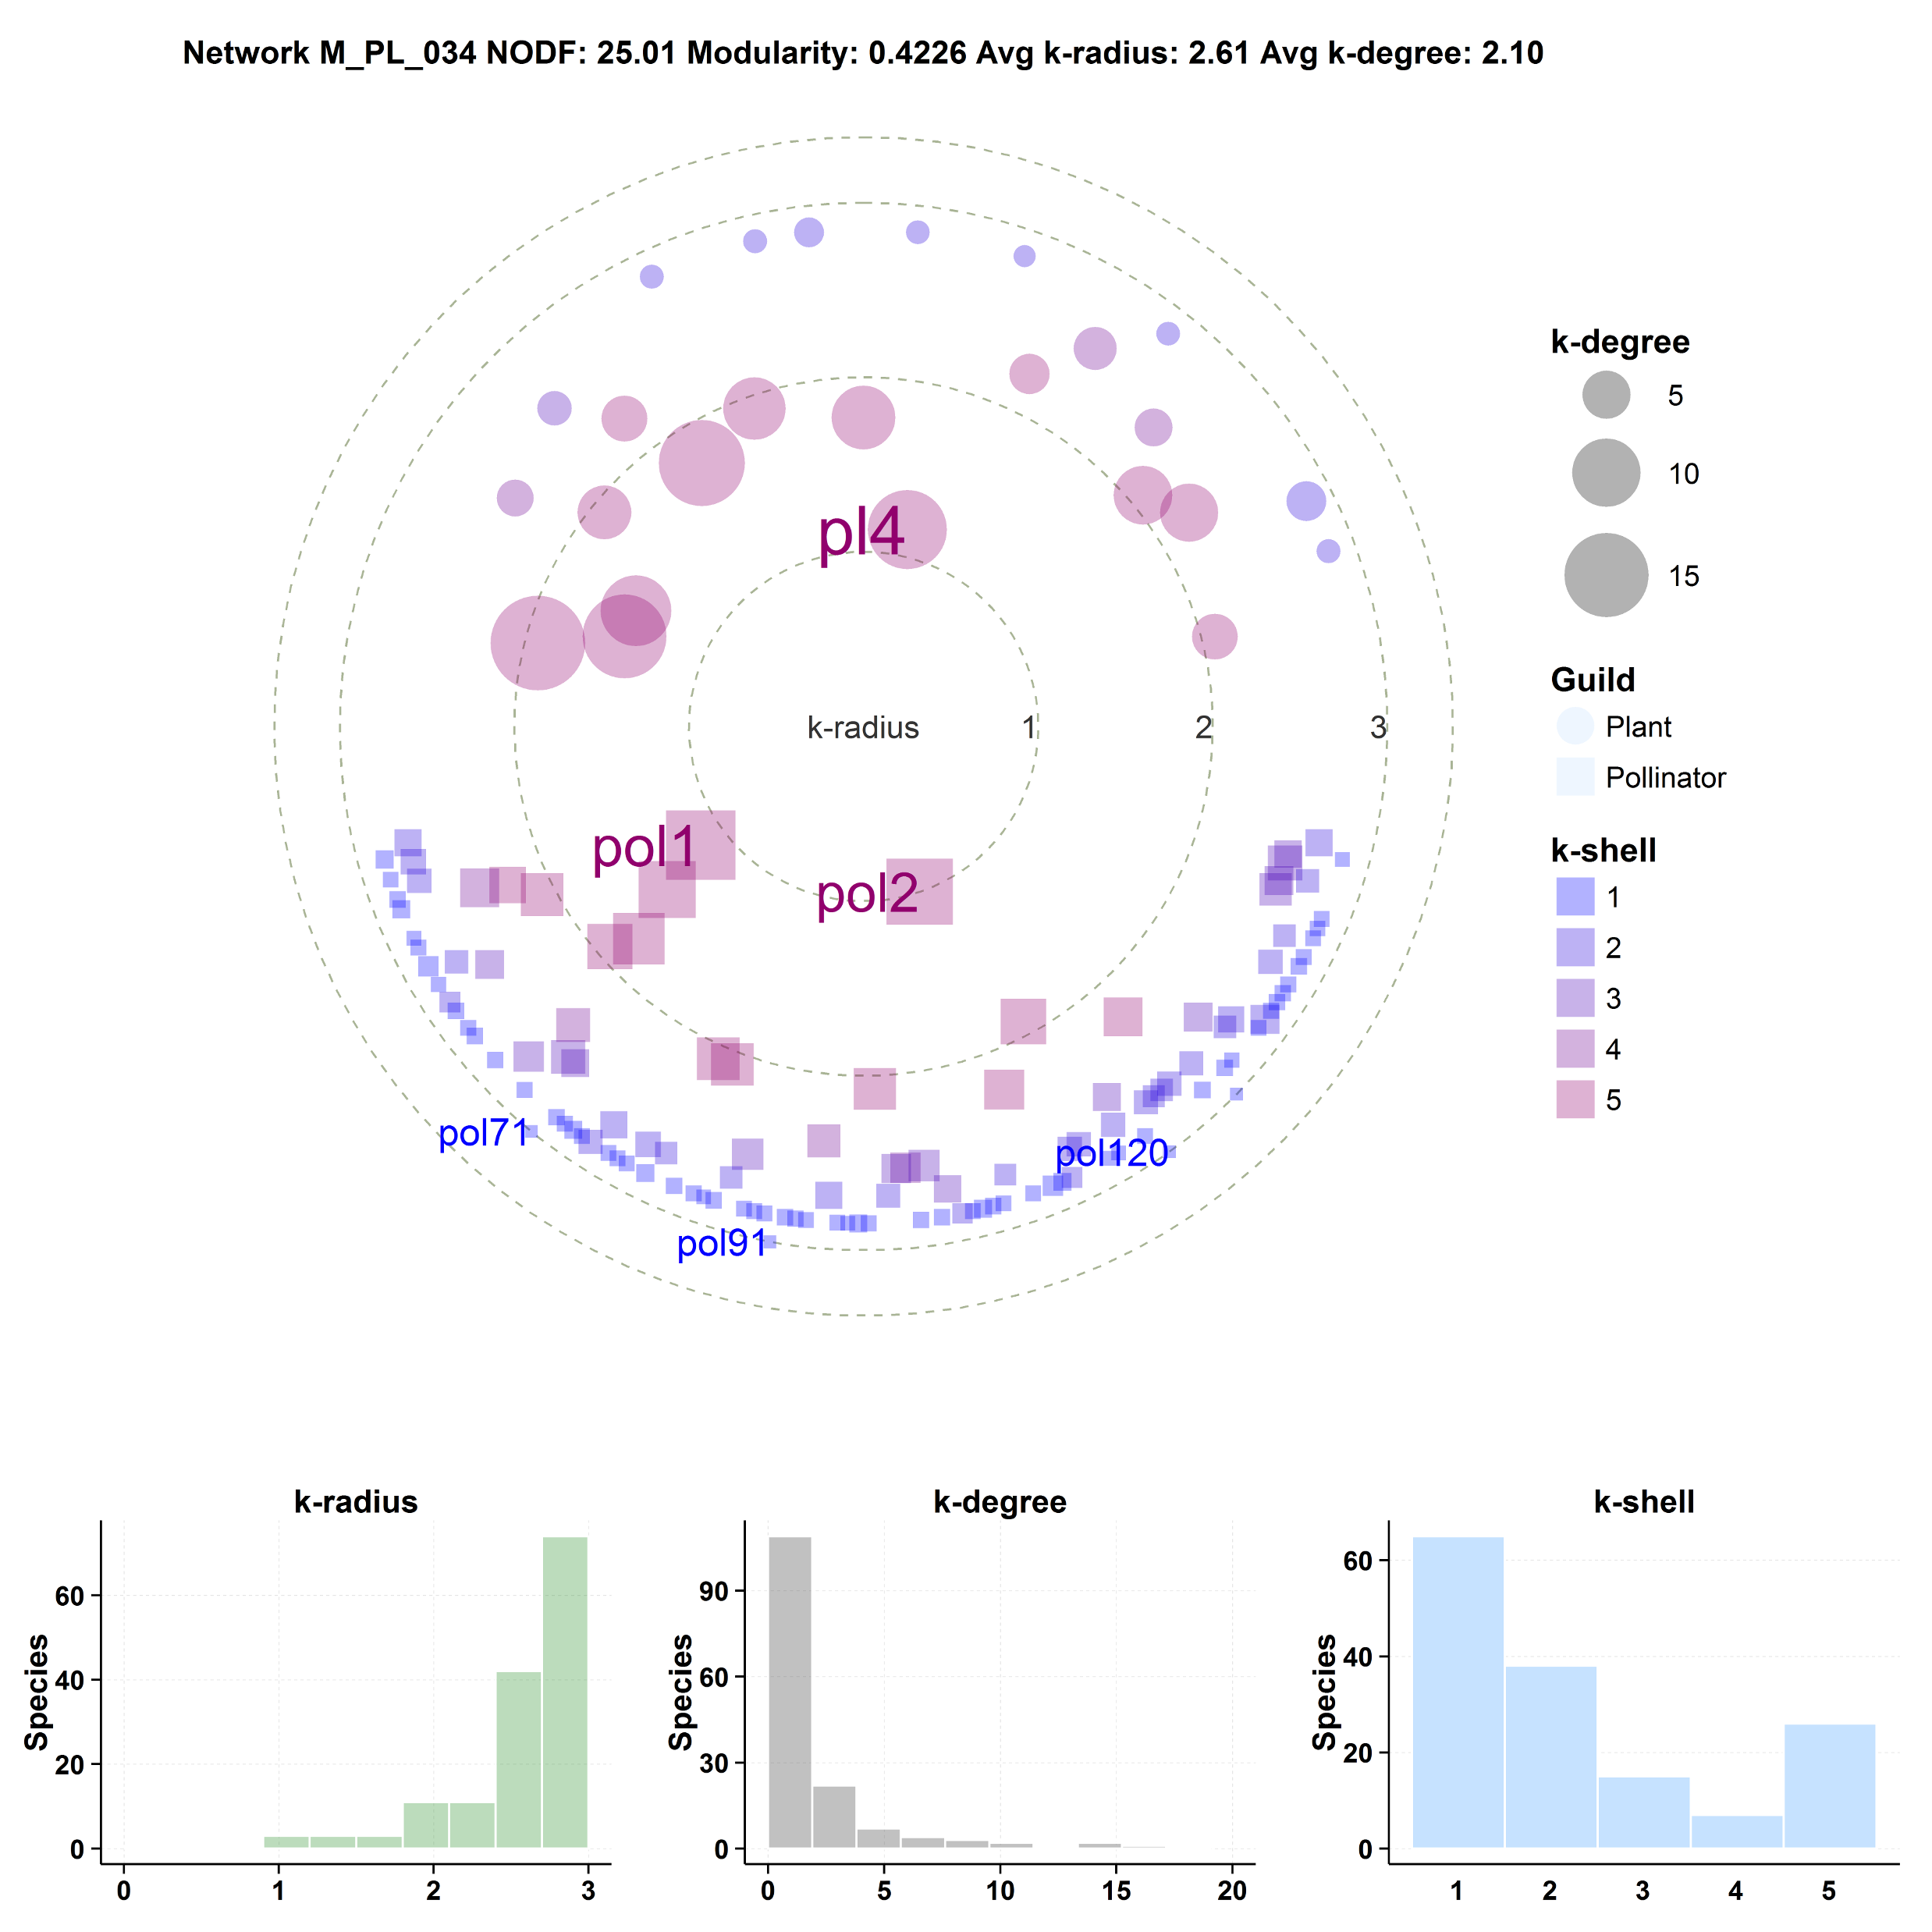
\includegraphics[scale=0.6]{Figures/VIS_M_PL_034_polar.png}
\caption[PolarExample]{Diagrama polar de una comunidad de polinizadores en la isla de Chiloé (Chile) \cite{smith2005diversity}.}
\label{fig:VIS_M_PL_034_polar}
\end{figure}

En nuestro caso hemos conservado la idea del diagrama concéntrico y la coloración en función del \textit{k-shell}, pero el diagrama polar difiere en todo lo demás de los dos mencionados. Para empezar, la red es bipartita. Cada clase se sitúa en un de los semiplanos y se utiliza la forma de los nodos para remarcar esta diferencia. El centro de cada especie se sitúa a una distancia $k_{radius}$ del origen de coordenadas, recordemos que el valor mínimo de esta magnitud es $1$. El ángulo se distribuye al azar por el algoritmo de representación para evitar al máximo la superposición de nodos. El área es proporcional al $k_{degree}$ y el color, propio de la \textit{k-shell}. Los enlaces no se representan.

Se puede elegir incluir los nombres de todas las especies, de ninguna, o de un pequeño número, por defecto las tres más centrales y las tres más alejadas. Adicionalmente, el usuario puede elegir que se añadan los histogramas de las tres \textit{k-magnitudes}, que contienen información muy valiosa.

La figura \ref{fig:VIS_M_PL_034_polar} es la representación polar de una red de polinizadores, que hemos elegido por ser una red mutualista tipo tanto por tamaño, anidamiento, modularidad y valores de las \textit{k magnitudes}, todos ellos no demasiado alejados de la media (tabla \ref{table:table_results}). El histograma de la distribución por \textit{k shells} tiene forma de bañera, muy repetido en estas redes. Hay unos pocos nodos domninantes y centrales, de índice $k = 5$ y un número importante de especies en las \textit{shells exteriores}. Es una red de elevada asimetría ($0.66$, véase tabla \ref{table:table_rewiring}).

La utilidad del diagrama polar se descubre al comparar varias redes, incluso si son de tamaños muy dispares. En la figura \ref{fig:VIS_Modvskdegree3}, hemos escogido tres redes situadas en ambos extremos y en el centro del diagrama \ref{fig:ESTATICA_corrfigs} (derecha). La red de polinizadores $PL\_010$  tiene un valor de $Modularity$ bajo $(0.25)$, y alto el de $\overline {k}_{degree}$ $(4.57)$. El diagrama polar muestra la estructura en capas del mutualismo. Esta es mucho más evidente en la red $SD\_007$ ($Modularity:    0.28$, $\overline {k}_{degree}: 2.34$). La distribución de $\overline {k}_{degree}$ es mucho más abrupta, con dos especies muy dominantes. La imagen transmite la idea de ser una red con mayor organización jerárquica que $PL\_010$.

La red $PL\_021$ es grande y fuertemente modular ($Modularity: 0.57$, $\overline {k}_{degree}: 1.23$). La distribución de $\overline {k}_{degree}$ es aun más abrupta. Se ha incluido en la parte inferior izquierda, la distribución de densidades que ya aparecía en la figura \ref{fig:ESTATICA_density_plots} porque la escala logarítmica en el eje horizontal permite ver mejor las diferencias.

\begin{figure}[h!]
\centering
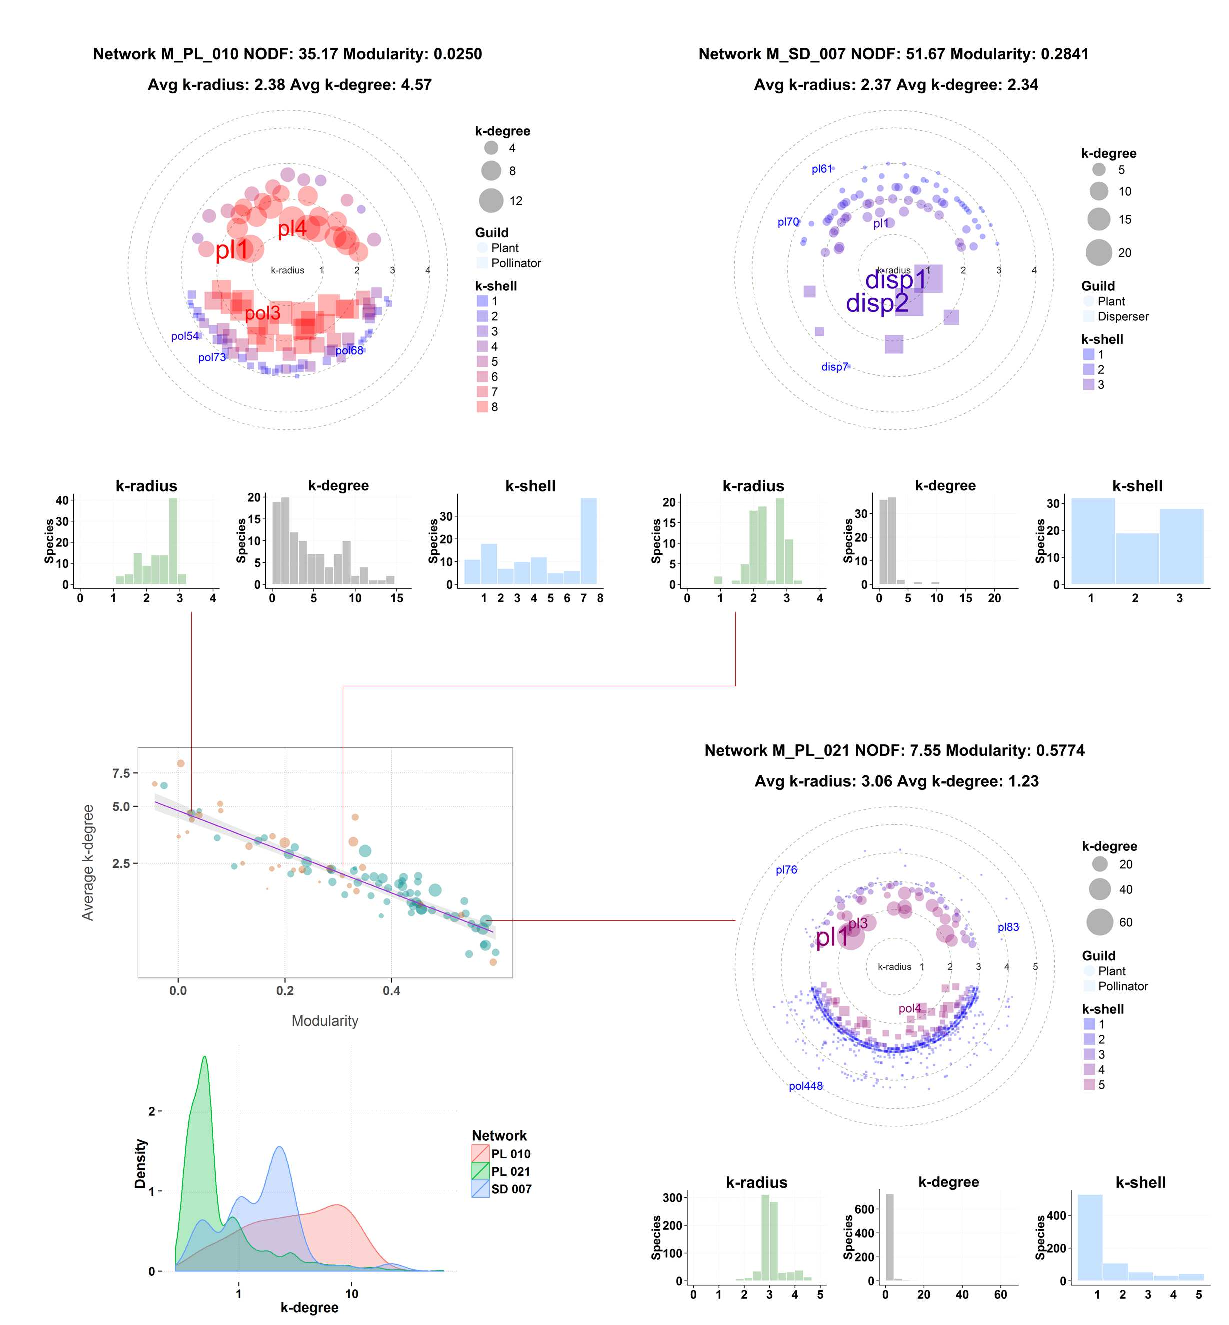
\includegraphics[scale=0.75]{Figures/VIS_Modvskdegree3.PDF}
\caption[PolarExample]{Comparación de tres redes mediante sus diagramas polares.}
\label{fig:VIS_Modvskdegree3}
\end{figure}

A pesar de que el diagrama polar ofrece una nueva visión de las comunidades mutualistas, tiene limitaciones. Como en toda estrategia de reducción de al información hay que renunciar a representar detalles en favor de una mejor visibilidad, en este caso los enlaces. No se trata de un detalle menor, así que se ha desarrollado un segundo tipo de diagrama que los toma como base de su construcción.

\subsection{El diagrama zigurat}

El diagrana zigurat se ha creado para mostrar la estructura de \textit{k shells} de una red bipartita y todos los enlaces entre sus nodos. La idea básica consiste en agrupar las especies en \textit{shells} que se representan como pequeños zigurats(\footnote{Según el DRAE: Torre escalonada y piramidal, característica de la arquitectura religiosa asiria y caldea.}). Las dos \textit{shells} máximas se colocan en el eje de simetría horizontal, ligeramente hacia la izquierda. El resto, se distribuyen siguiendo una disposición en forma de almendra, que deja un gran espacio libre para dibujar los enlaces.

\begin{figure}[h!]
\centering
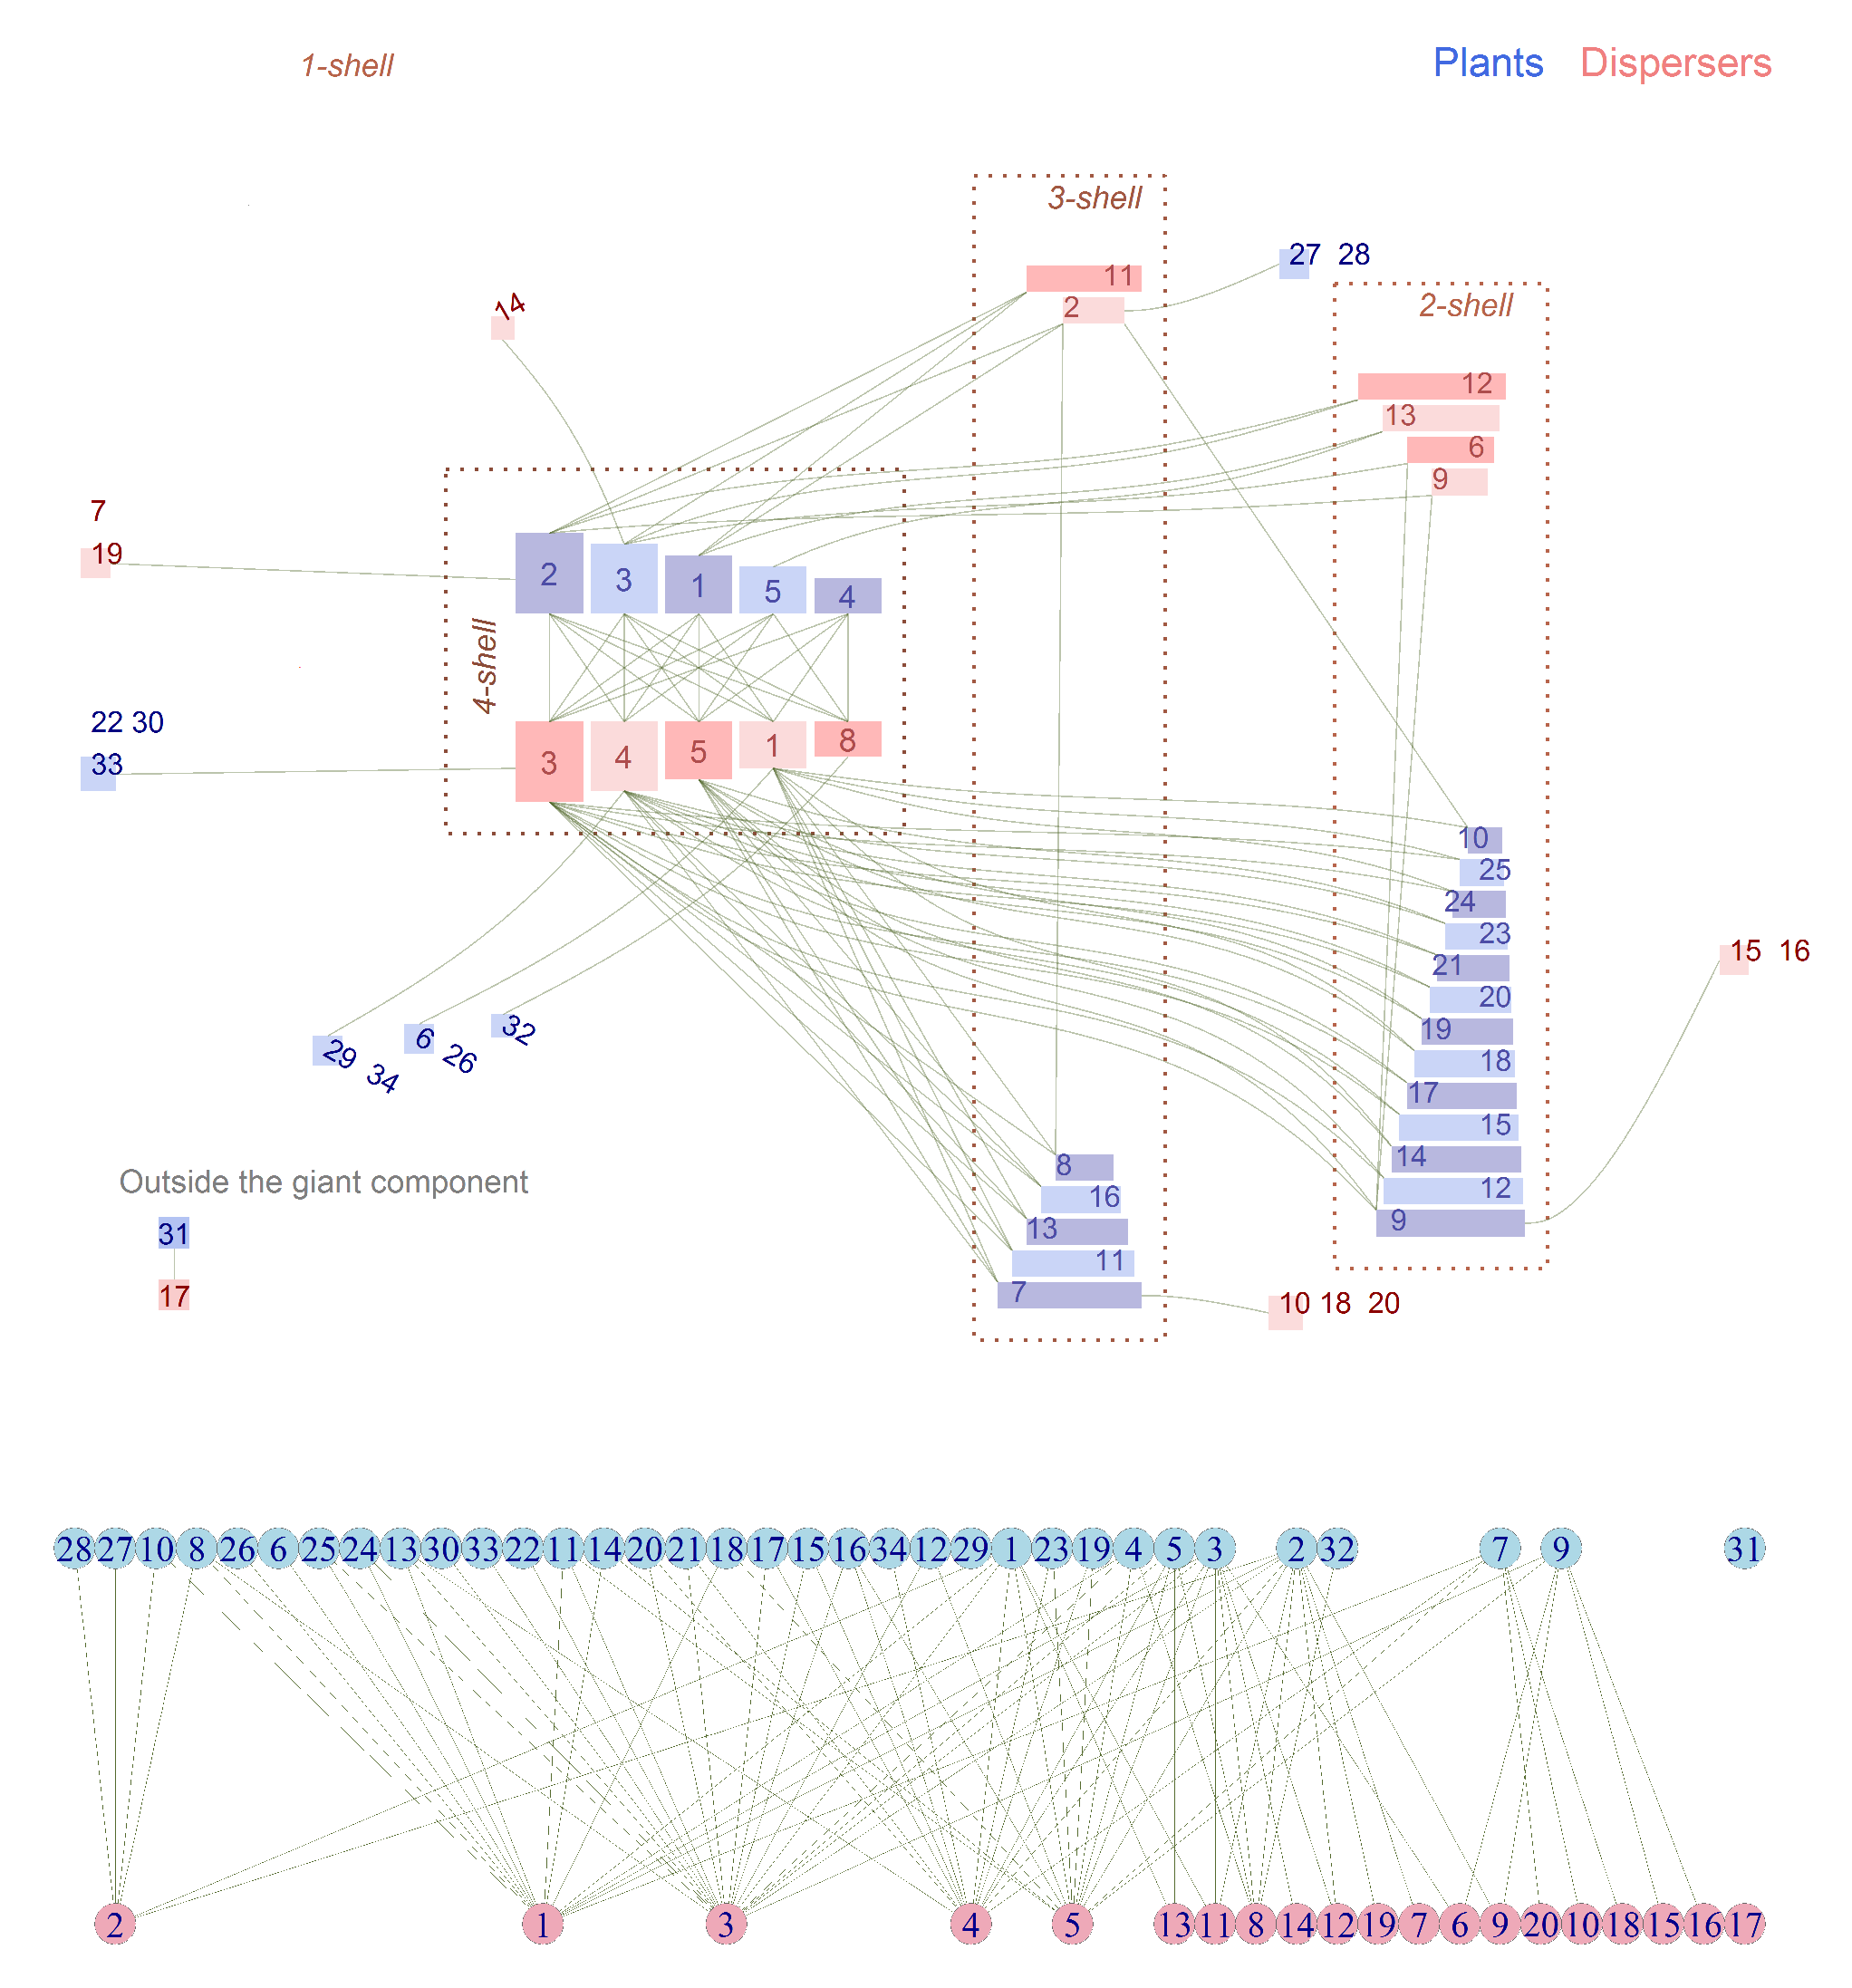
\includegraphics[scale=0.45]{Figures/VIS_ALL_SD_004.eps}
\caption {Diagrama zigurat de una comunidad de aves frugívoras de Puerto Rico, con $54$ especies y $95$ enlaces \cite{carlo2003avian}. $\overline k_{radius} = 2,19$, $\overline k_{degree} = 2,37$, $NODF = 39,82$, $Modularity = 0.34$. Abajo el diagrama bipartito.}
\label{fig:ziggurat}
\end{figure}

En la \textit{shell} máxima las especies se ordenan por $k_{degree}$, con el valor mayor a la izquierda. En el resto, se ordenan por $k_{radius}$, correspondiendo la base del zigurat a la especie de menor $k_{radius}$.

Las especies de la \textit{1-shell} se disponen como una nube el torno a la almendra central. Si, como sucede a menudo, varias especies de esta \textit{shell} comparten enlace, se dibujan de forma agrupada y con un único enlace.

En algunas redes, los autores han incluido observaciones de especies que no están conectadas con la componente gigante. En ese caso, se representa el fragmento inconexo, pero no se tiene en cuenta para la \textit{k descomposición}.

Por último, es importante recalcar que en el diagrama zigurat, las áreas no transmiten información sobre tamaños de la población.

La red de la figura \ref{fig:ziggurat} es de pequeño tamaño. En el gráfico bipartito todavía se pueden seguir los enlaces individuales. Sin embargo, el zigurat ofrece una visión mucho más rica de la organización con cuatro \textit{shells} internas y una pequeña \textit{1-shell}. Se pueden descubrir con facilidad algunos patrones, como la baja conectividad entre especies de las \textit{shells} de menor índice $k$, o la relativa importancia de la especie dispersora $2$ que en el bipartito aparece en el extremo izquierdo.

\begin{figure}[ht!]
\centering
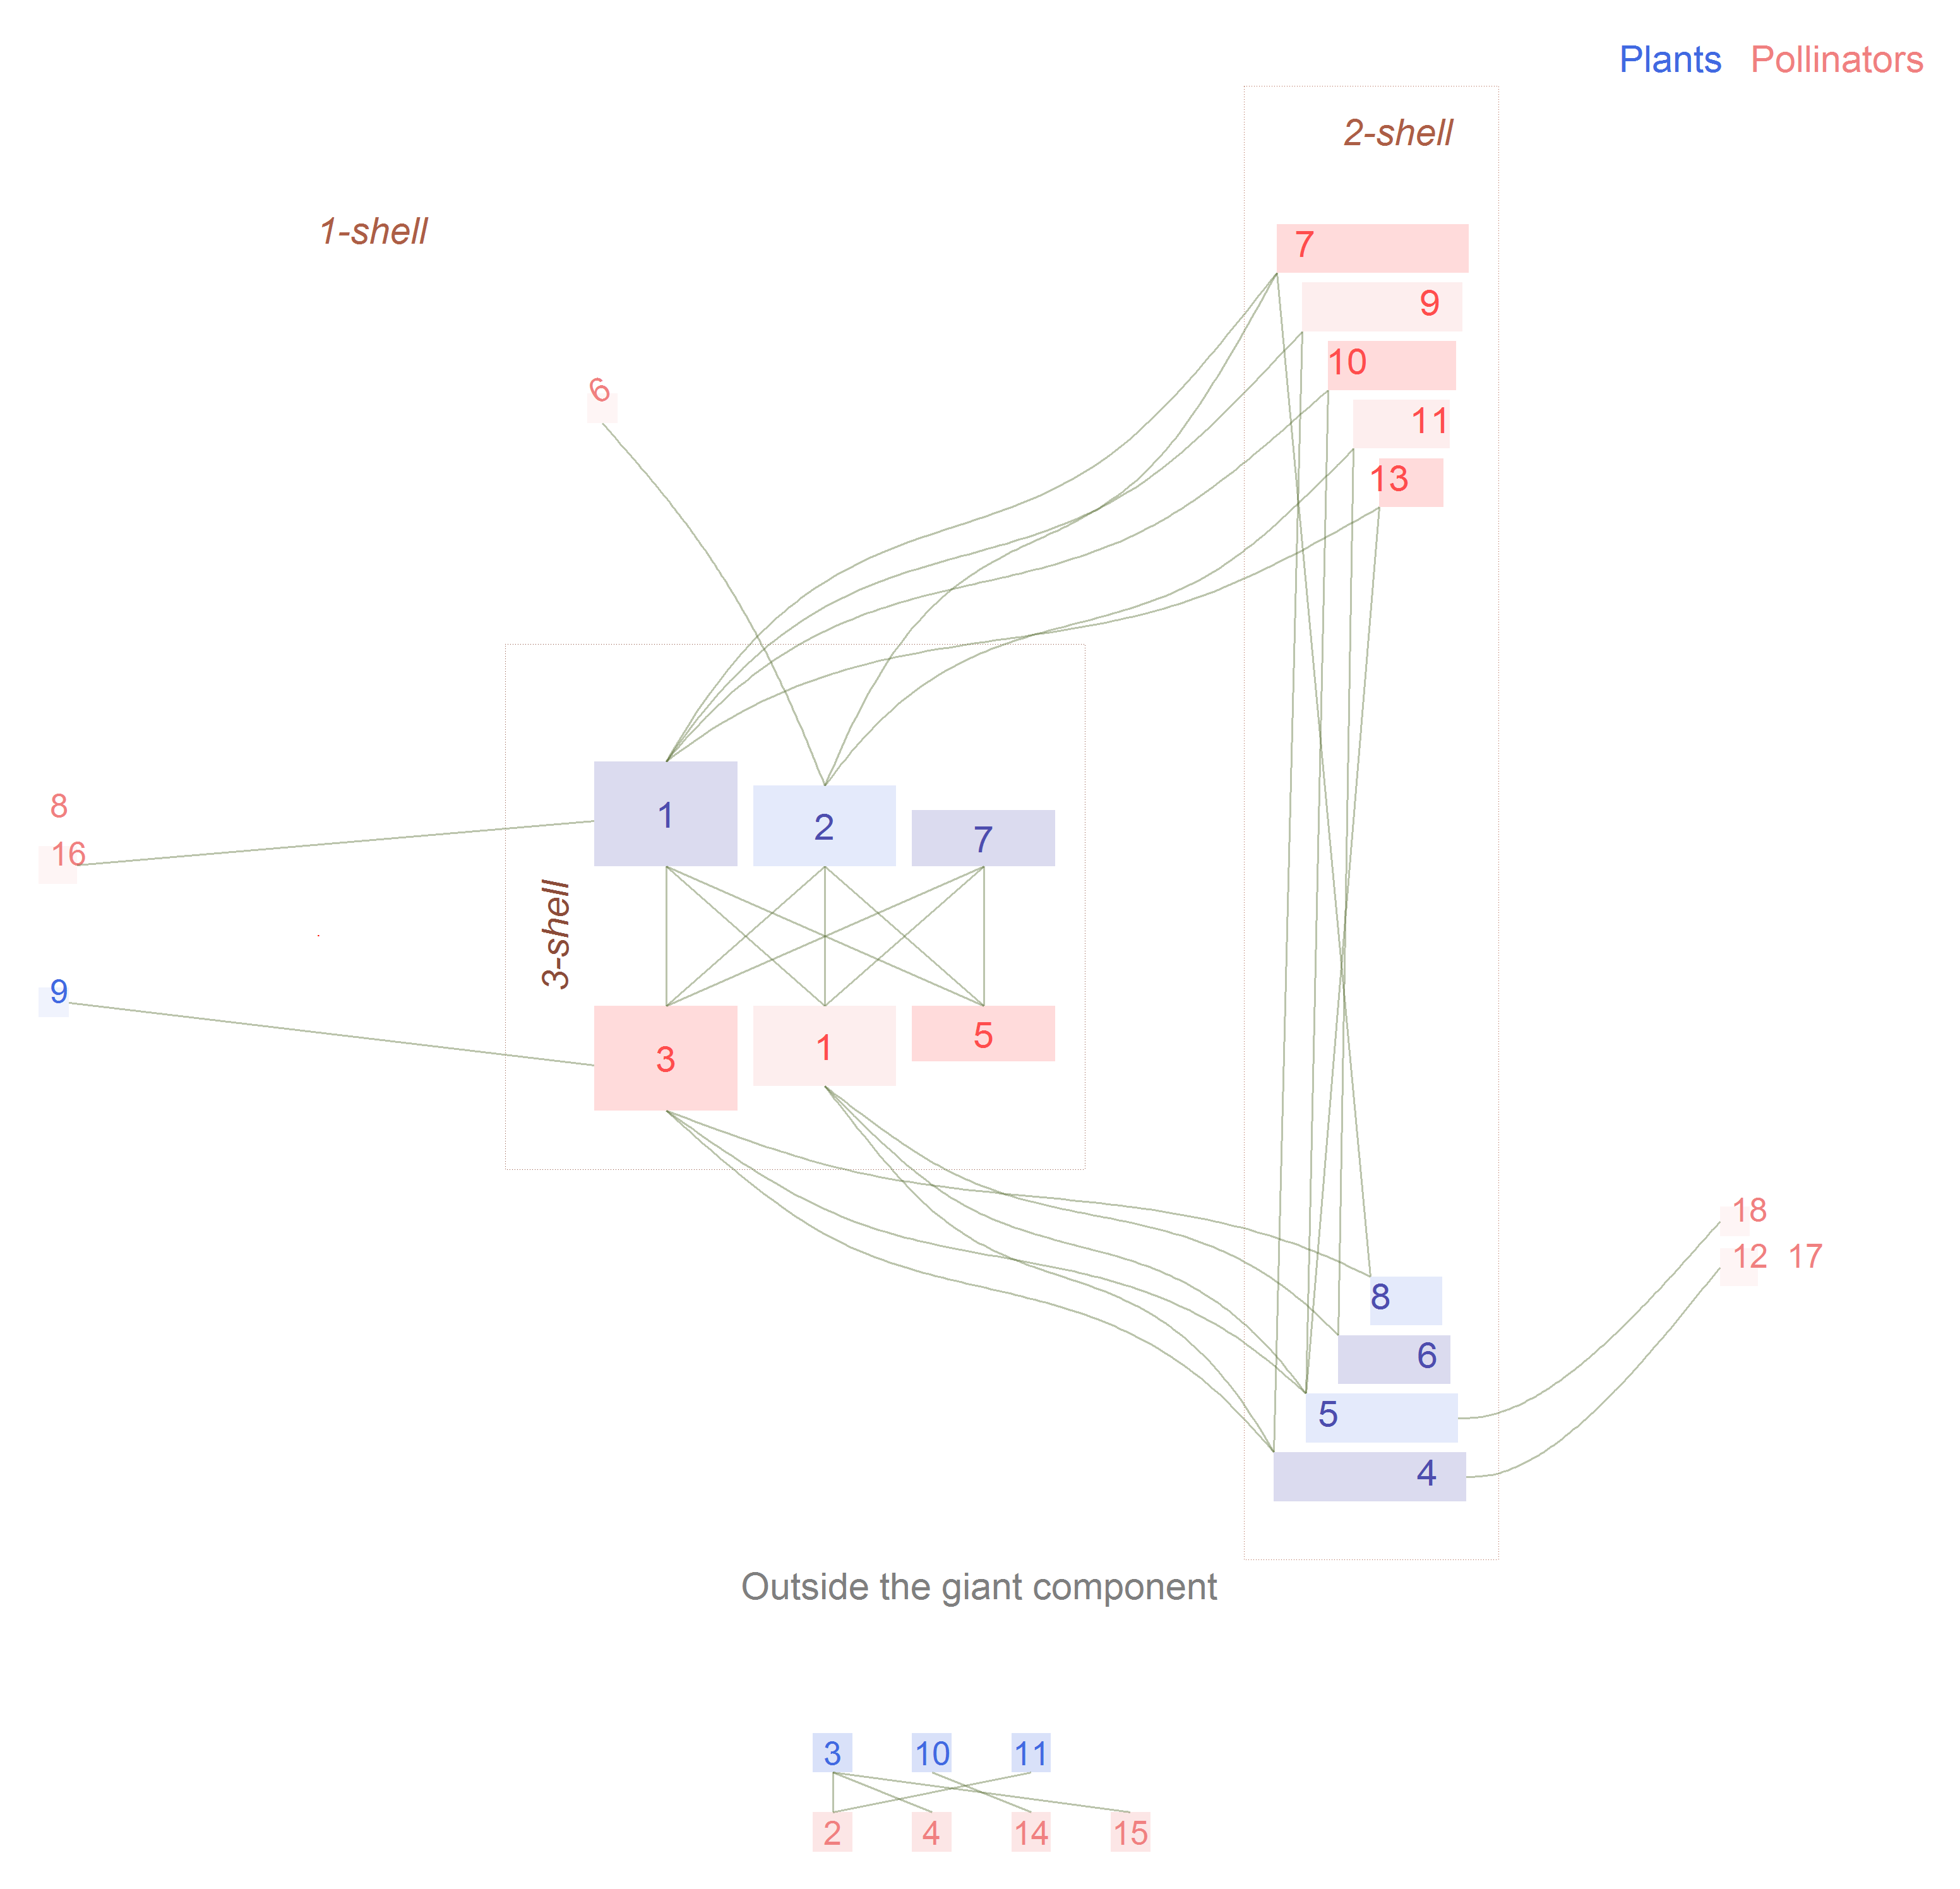
\includegraphics[scale=0.16]{Figures/VIS_zig_pl_024.png}
\caption {Red de polinizadores $M\_PL\_010$, Melville Island, Canada \cite{mosquin1967observations}, con $29$ especies y $38$ enlaces}
\label{fig:VIS_zig_pl_024}
\end{figure}

El diagrama zigurat funciona bien para los tamaños típicos de las redes mutualistas documentadas en la literatura. La red de la figura \ref{fig:VIS_zig_pl_024} es pequeña, muy simétrica y con valores intermedios de $NODF$ y de las \textit{k magnitudes} (véase la tabla \ref{table:table_results}). La especie con mayor $k_{degree}$ $(5,74)$ es la planta $1$. En esta red todas las especies de las \textit{shells} máximas están conectactas entre sí, por lo que sus $k_{radius}$ valen $1,0$, pero esto no tiene por qué suceder siempre. Las más distantes de la $3$-$shell$ (descartando a las que no están conectadas con la componente gigantes) son los polinizdores $12$,$17$ y $18$, con  $k_{radius}$ $3,0$, que aparecen conectadas en el extremo derecho al zigurat de la $2$-$shell$ de plantas.


\begin{figure}[h!]
\centering
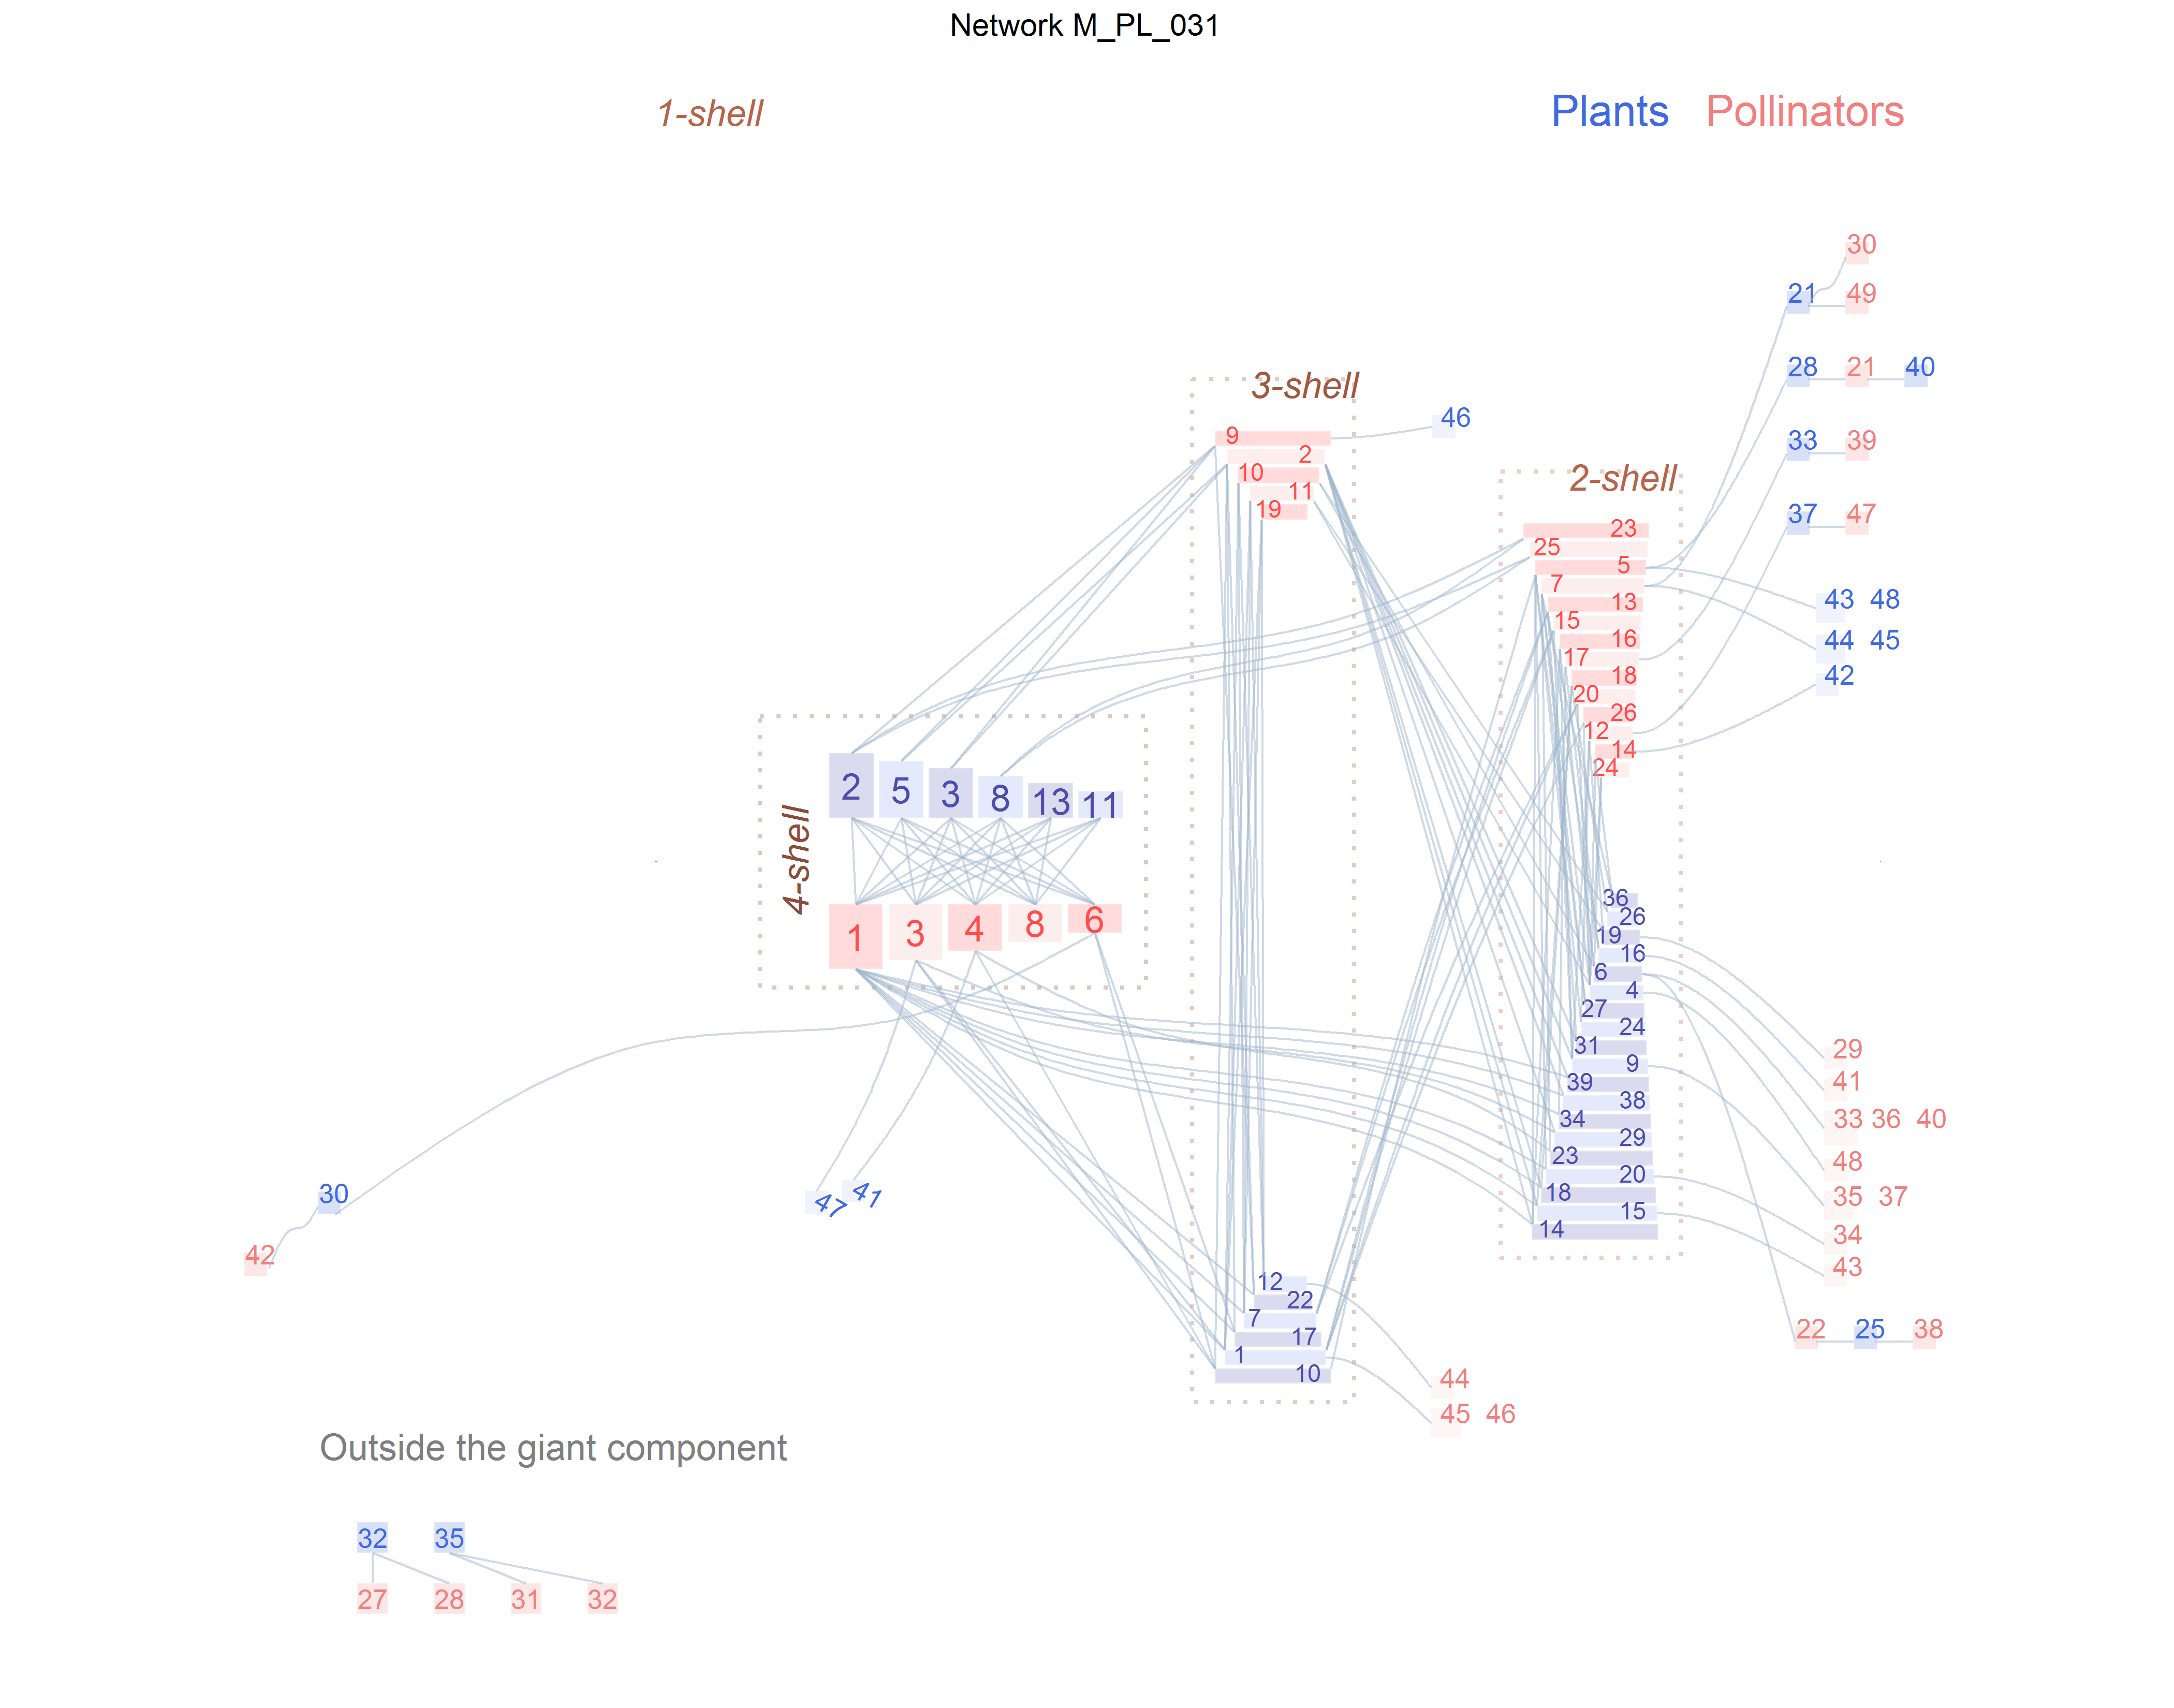
\includegraphics[scale=0.14]{Figures/VIS_M_PL_031_ziggurat.png}
\caption {Red de polinizadores $M\_PL\_031$ del Parque Nacional de Canaima, Venezuela, con $97$ especies y $156$ enlaces \cite{ramirez1989biologia}.}
\label{fig:VIS_M_PL_031_ziggurat}
\end{figure}

La red de la figura \ref{fig:VIS_M_PL_031_ziggurat} es de un tamaño intermedio, y muestra abundancia de especialistas conectadas a otras especialistas, una circunstancia poco común. A diferencia del caso anterior, no todas las especies del las \textit{shells} máximas tienen enlaces directos con todas las de la clasetaria c con. Así, mientras el $k_{radius}$ del polinizador $1$ o la planta $2$ es $1,0$, el de la planta $13$ es $1,4$ y el del polinizador $6$ es $1.66$ (tabla \ref{table:kmag_pl_031}). La existencia de especialistas ultraperiféricos se traduce en valores elevados del $k_{radius}$, por ejemplo $7.0$ para el polinizador $38$ o $6.2$ para la planta $25$ que es el primer enlace de su camino más corto hacia el centro de la red.

\begin{figure}[ht!]
\centering
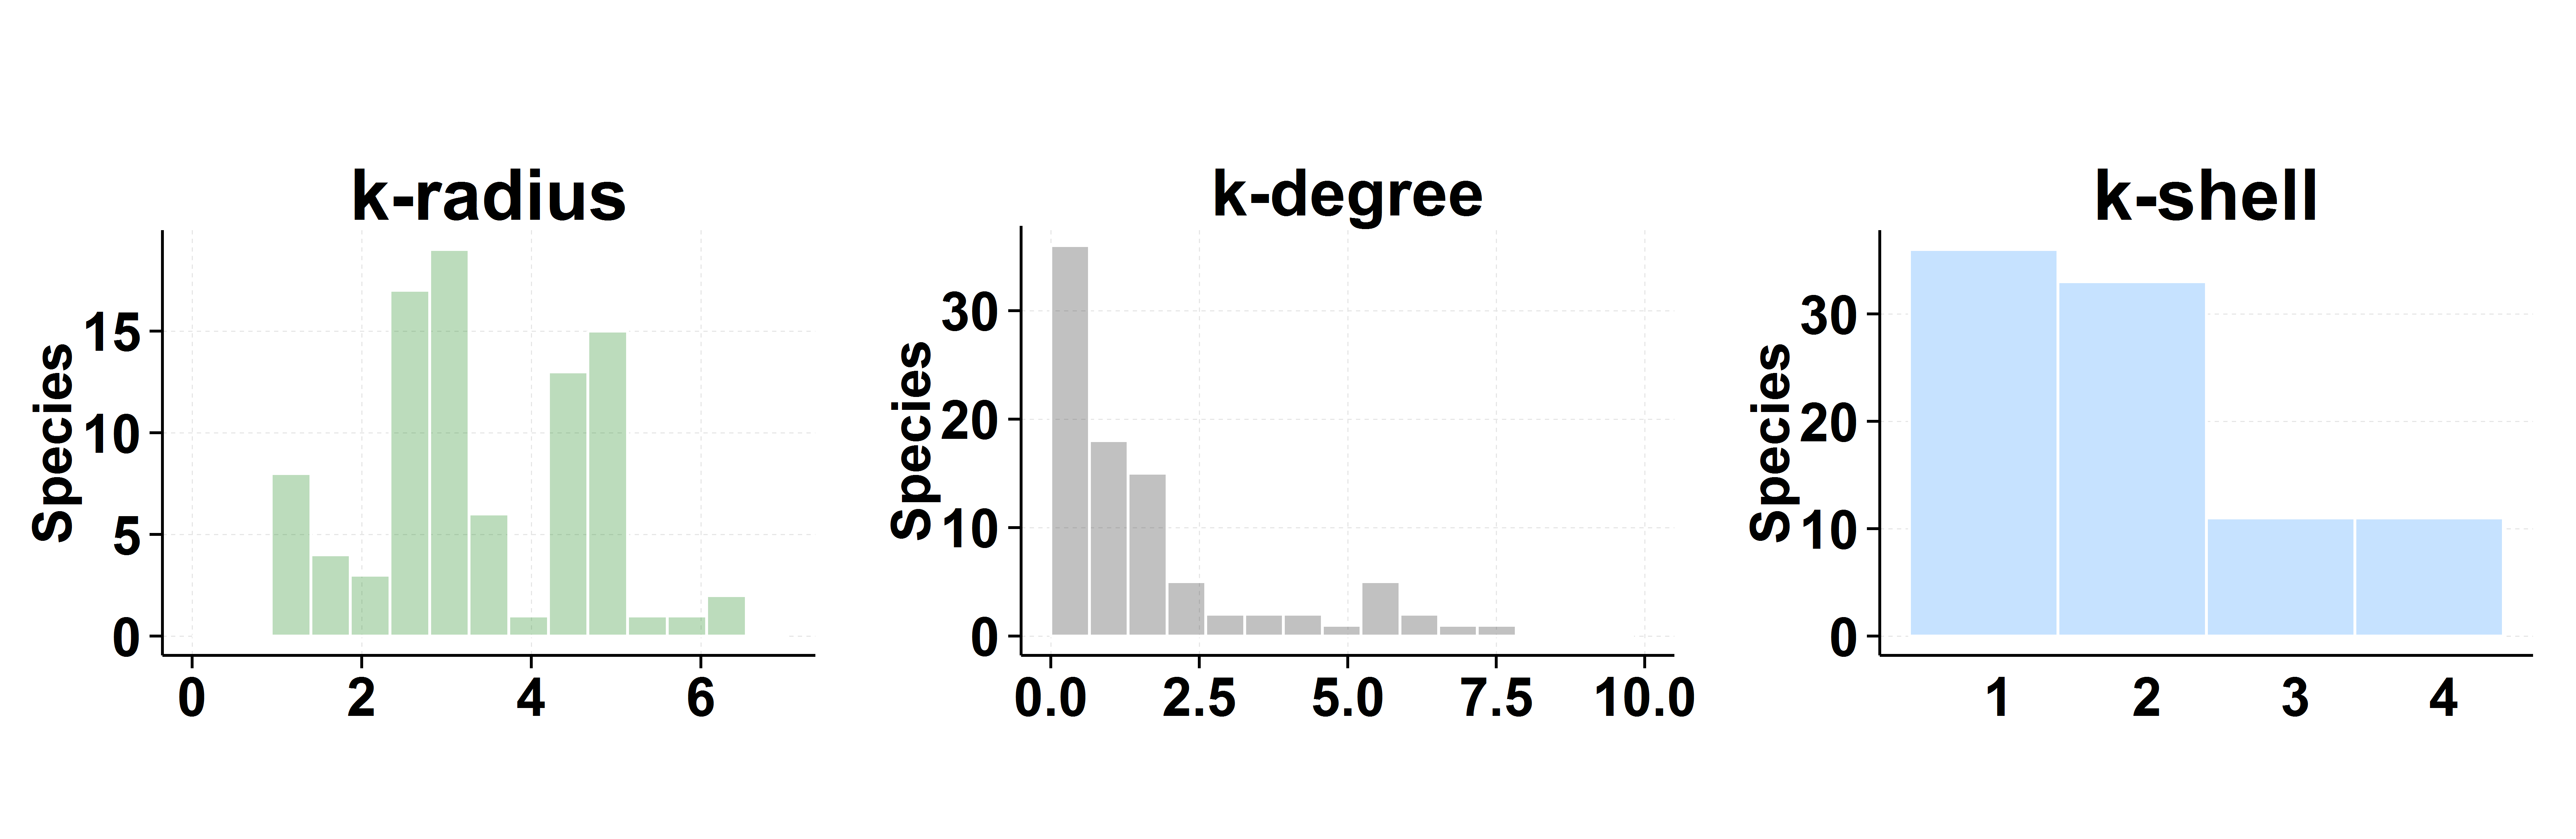
\includegraphics[scale=0.45]{Figures/VIS_M_PL_031_polar.png}
\caption {Histograma de las \textit{k magnitudes} de polinizadores del Parque Nacional de Canaima, Venezuela \cite{ramirez1989biologia}.}
\label{fig:VIS_M_PL_031_polar}
\end{figure}

Estas especies tan alejadas del centro corren el peligro de extinción por arrastre que se describió en el apartado \ref{results_K_constante}. Supongamos que el polinizador número $7$ se extingue por una plaga. En la parte superior derecha de la figura \ref{fig:VIS_M_PL_031_ziggurat} puede verse la tripleta planta $21$, polinizadores $30$ y $49$ que quedarían desconectados de la componente gigante y posiblemente se extinguirían también. En el mejor de los casos, si por el peso de sus enlaces superaran el mínimo vital de la nueva red formada por las tres, podrían sobrevivir aisladas pero mucho más expuestas a cualquier perturbación posterior. Las plantas $44$ y $45$ desaparecerían con seguridad porque el polinizador $7$ es su única especie benefactora. De esta manera, la destrucción de un polinizador podría arrastrar cinco especies más a la extinción. En el diagrama se puede ver también la gran conectividad entre especies de las \textit{shells} de índices $2$ y $3$, que se refleja en un anidamiento bajo y notable modularidad. La red de la figura \ref{fig:ziggurat} es mucho más anidada, con pocos enlaces que no terminen en la $4$-$shell$ y con un $\overline k_{radius}$ reducido ($2,19$ frente a $3,39$).


El tamaño de una red se puede medir en número de nodos o en número de enlaces, pero es esta segunda cifra la que predomina a la hora de fijar la complejidad de la estructura de \textit{k shells}. La red de la figura \ref{fig:VIS_M_PL_010_ziggurat}, tiene $107$ especies y $456$ enlaces y su índice $k$ máximo es $8$. Se aprecia asimetría importante con predominio de los polinzadores. En contraste con los ejemplos anteriores, hay muy pocas especies que pertenezcan a la $1$-$shell$. Las conexiones entre las distintas \textit{shells} forman un entramado visualmente complejo.

Con menos especies $(85)$ y solo un $10\%$ más de enlaces, la comunidad de frugívoros de la selva malaya de la figura \ref{fig:VIS_M_PL_047_ziggurat}, tiene un índice $k$ máximo de $11$, ninguna otra de la colección \textit{web of life} lo alcanza. Es muy asimétrica y fuertemente anidada $(NODF = 58,84)$. El valor de $\overline k_{degree}$ es excepcional, $8,4$, por la circunstancia de tener ese $k$ máximo, la elevada conectividad de las especies y su cercanía a las \textit{k shells} $11$.

La red de polinizadores de un brezal danés (figura \ref{fig:VIS_M_PL_047_ziggurat}), tiene $205$ especies y $425$ enlaces. El $k$ máximo es solo $6$. La asimetría es también muy marcada pero lo que más destaca es la extraordinaria cantidad de polinizadores en la $1$-$shell$. Con este ejemplo se aprecia mejor el valor de agrupar todas las especies de la $1$-$shell$ que se conectan a una especie de las \textit{shells} más internas y dibujar solo un enlace. 

\clearpage

% Table generated by Excel2LaTeX from sheet 'pl31_indiv'
\begin{table}[htbp]
\small
  \centering

    \begin{tabular}{lrrrlrr}
    \toprule
    Especie & $k_{radius}$ & $k_{degree}$ &      & Especie & $k_{radius}$ & $k_{degree}$ \\
    \midrule
    Planta1 & 2,20 & 5,00 &      & Polinizador1 & 1,00 & 9,80 \\
    Planta2 & 1,00 & 5,96 &      & Polinizador2 & 2,33 & 6,37 \\
    Planta3 & 1,00 & 5,53 &      & Polinizador3 & 1,00 & 7,21 \\
    Planta4 & 3,80 & 1,93 &      & Polinizador4 & 1,00 & 6,75 \\
    Planta5 & 1,00 & 5,53 &      & Polinizador5 & 3,00 & 2,80 \\
    Planta6 & 4,20 & 1,67 &      & Polinizador6 & 1,67 & 5,39 \\
    Planta7 & 2,60 & 3,00 &      & Polinizador7 & 3,00 & 1,81 \\
    Planta8 & 1,00 & 5,46 &      & Polinizador8 & 1,00 & 5,43 \\
    Planta9 & 3,00 & 1,79 &      & Polinizador9 & 2,00 & 3,72 \\
    Planta10 & 1,80 & 3,36 &      & Polinizador10 & 3,00 & 1,55 \\
    Planta11 & 1,40 & 4,00 &      & Polinizador11 & 3,00 & 1,58 \\
    Planta12 & 4,20 & 1,20 &      & Polinizador12 & 4,33 & 1,07 \\
    Planta13 & 1,40 & 4,00 &      & Polinizador13 & 3,00 & 1,41 \\
    Planta14 & 2,60 & 2,10 &      & Polinizador14 & 5,00 & 0,65 \\
    Planta15 & 2,60 & 2,10 &      & Polinizador15 & 3,00 & 1,17 \\
    Planta16 & 4,20 & 0,87 &      & Polinizador16 & 3,00 & 0,96 \\
    Planta17 & 2,20 & 2,03 &      & Polinizador17 & 3,00 & 0,84 \\
    Planta18 & 2,60 & 1,76 &      & Polinizador18 & 3,00 & 1,01 \\
    Planta19 & 4,20 & 0,76 &      & Polinizador19 & 3,00 & 1,08 \\
    Planta20 & 2,60 & 1,67 &      & Polinizador20 & 3,00 & 1,10 \\
    Planta21 & 4,60 & 0,73 &      & Polinizador21 & 5,00 & 0,48 \\
    Planta22 & 2,60 & 1,93 &      & Polinizador22 & 5,00 & 0,40 \\
    Planta23 & 2,60 & 1,33 &      & Polinizador23 & 2,33 & 2,00 \\
    Planta24 & 3,40 & 0,56 &      & Polinizador24 & 5,00 & 0,50 \\
    Planta25 & 6,20 & 0,34 &      & Polinizador25 & 2,33 & 2,00 \\
    Planta26 & 4,20 & 0,67 &      & Polinizador26 & 3,00 & 0,72 \\
    Planta27 & 3,40 & 0,67 &      & Polinizador27 & *    & * \\
    Planta28 & 3,40 & 0,53 &      & Polinizador28 & *    & * \\
    Planta29 & 2,60 & 1,43 &      & Polinizador29 & 5,00 & 0,24 \\
    Planta30 & 2,60 & 0,87 &      & Polinizador30 & 5,00 & 0,22 \\
    Planta31 & 3,00 & 0,76 &      & Polinizador31 & *    & * \\
    Planta32 & *    & *    &      & Polinizador32 & *    & * \\
    Planta33 & 4,60 & 0,53 &      & Polinizador33 & 5,00 & 0,24 \\
    Planta34 & 2,60 & 1,33 &      & Polinizador34 & 3,00 & 0,38 \\
    Planta35 & *    & *    &      & Polinizador35 & 4,33 & 0,33 \\
    Planta36 & 4,60 & 0,53 &      & Polinizador36 & 5,00 & 0,24 \\
    Planta37 & 5,00 & 0,39 &      & Polinizador37 & 4,33 & 0,33 \\
    Planta38 & 2,60 & 1,43 &      & Polinizador38 & 7,00 & 0,16 \\
    Planta39 & 2,60 & 1,43 &      & Polinizador39 & 5,00 & 0,22 \\
    Planta40 & 5,40 & 0,20 &      & Polinizador40 & 5,00 & 0,24 \\
    Planta41 & 2,60 & 1,00 &      & Polinizador41 & 5,00 & 0,24 \\
    Planta42 & 5,80 & 0,20 &      & Polinizador42 & 3,67 & 0,38 \\
    Planta43 & 3,40 & 0,33 &      & Polinizador43 & 3,00 & 0,38 \\
    Planta44 & 4,60 & 0,33 &      & Polinizador44 & 5,00 & 0,24 \\
    Planta45 & 4,60 & 0,33 &      & Polinizador45 & 3,00 & 0,45 \\
    Planta46 & 3,00 & 0,50 &      & Polinizador46 & 3,00 & 0,45 \\
    Planta47 & 2,60 & 1,00 &      & Polinizador47 & 6,33 & 0,20 \\
    Planta48 & 3,40 & 0,33 &      & Polinizador48 & 5,00 & 0,26 \\
         &      &      &      & Polinizador49 & 5,00 & 0,22 \\
    \bottomrule
    \end{tabular}%
    \caption{\label{table:kmag_pl_031} \textit{k magnitudes} de la red  de polinizadores $M\_PL\_031$ del Parque Nacional de Canaima, Venezuela, \cite{ramirez1989biologia}. Valores globales: $\overline k_{radius} = 3,39$; $\overline k_{degree} = 1,57$. Las especies desconectadas de la componente gigante aparecen señaladas con asterisco.}
\end{table}%

\clearpage
\begin{figure}[ht!]
\centering
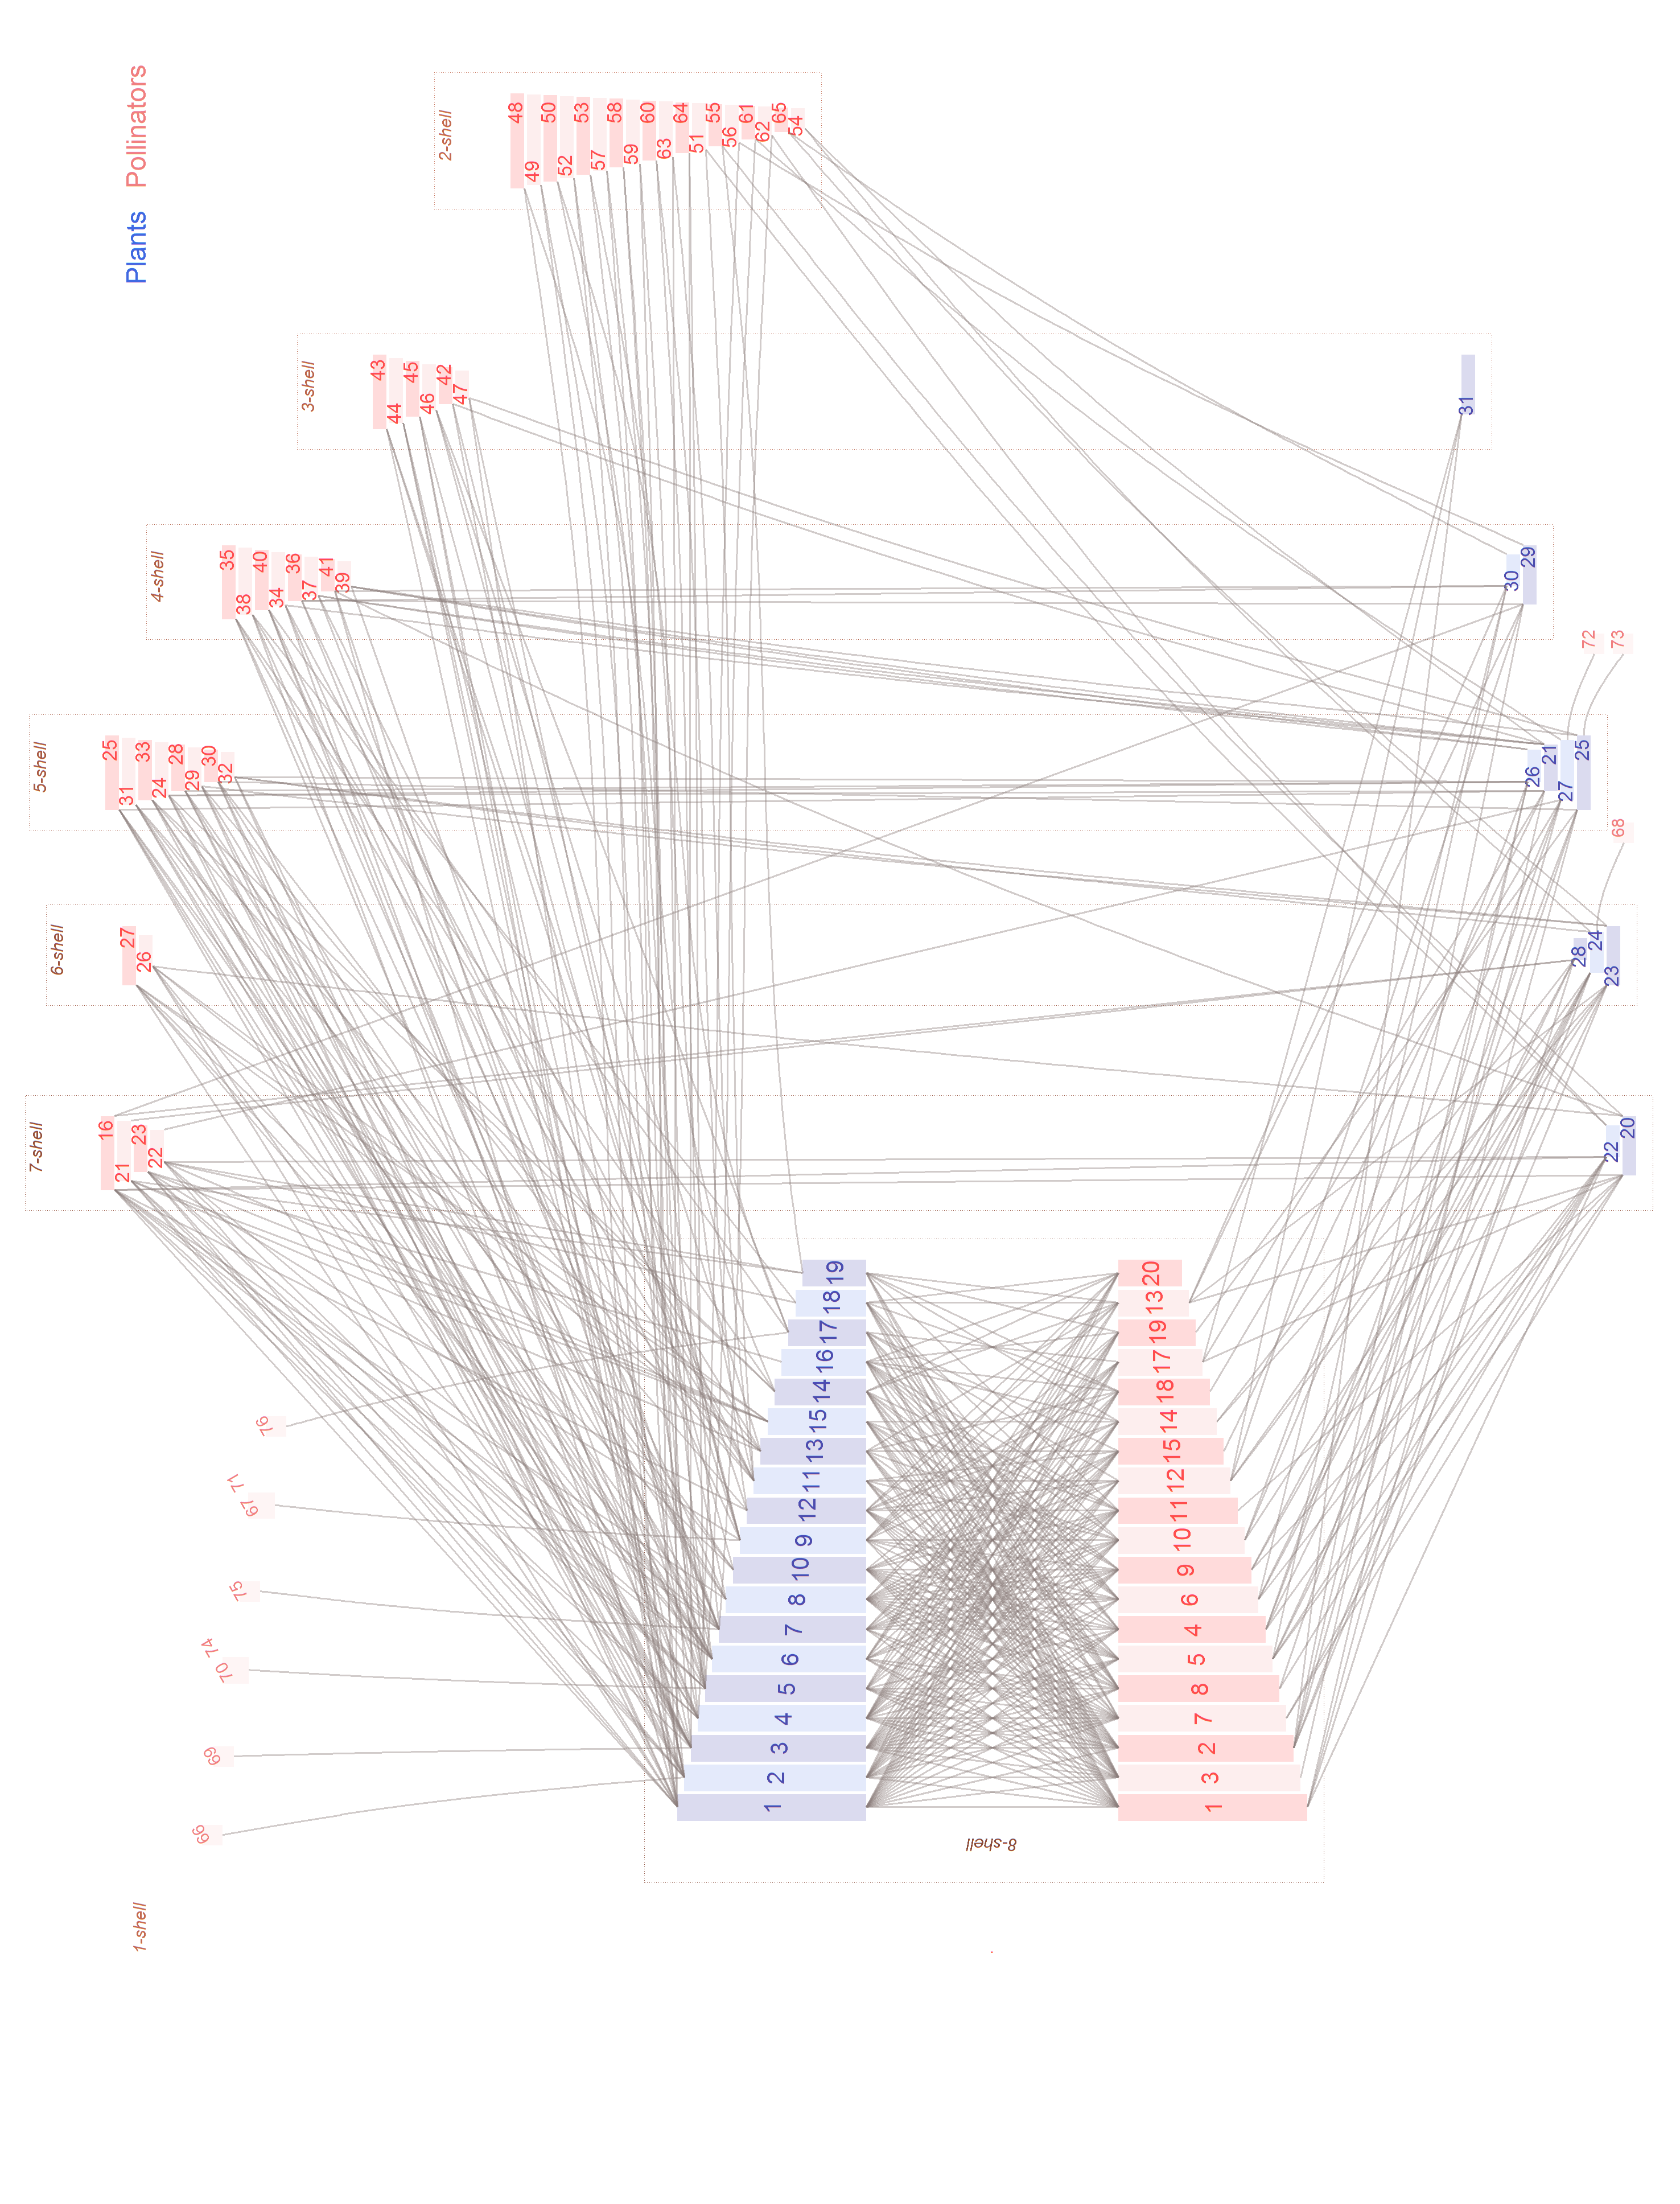
\includegraphics[scale=0.6]{Figures/VIS_M_PL_010_ziggurat.png}
\caption {Red de polinizadores $M\_PL\_010$ (Elberling \& Olesen, no publicada), con $107$ especies y $456$ enlaces. Su diagrama polar puede verse en la figura \ref{fig:VIS_Modvskdegree3}.}
\label{fig:VIS_M_PL_010_ziggurat}
\end{figure}

\clearpage
\begin{figure}[ht!]
\centering
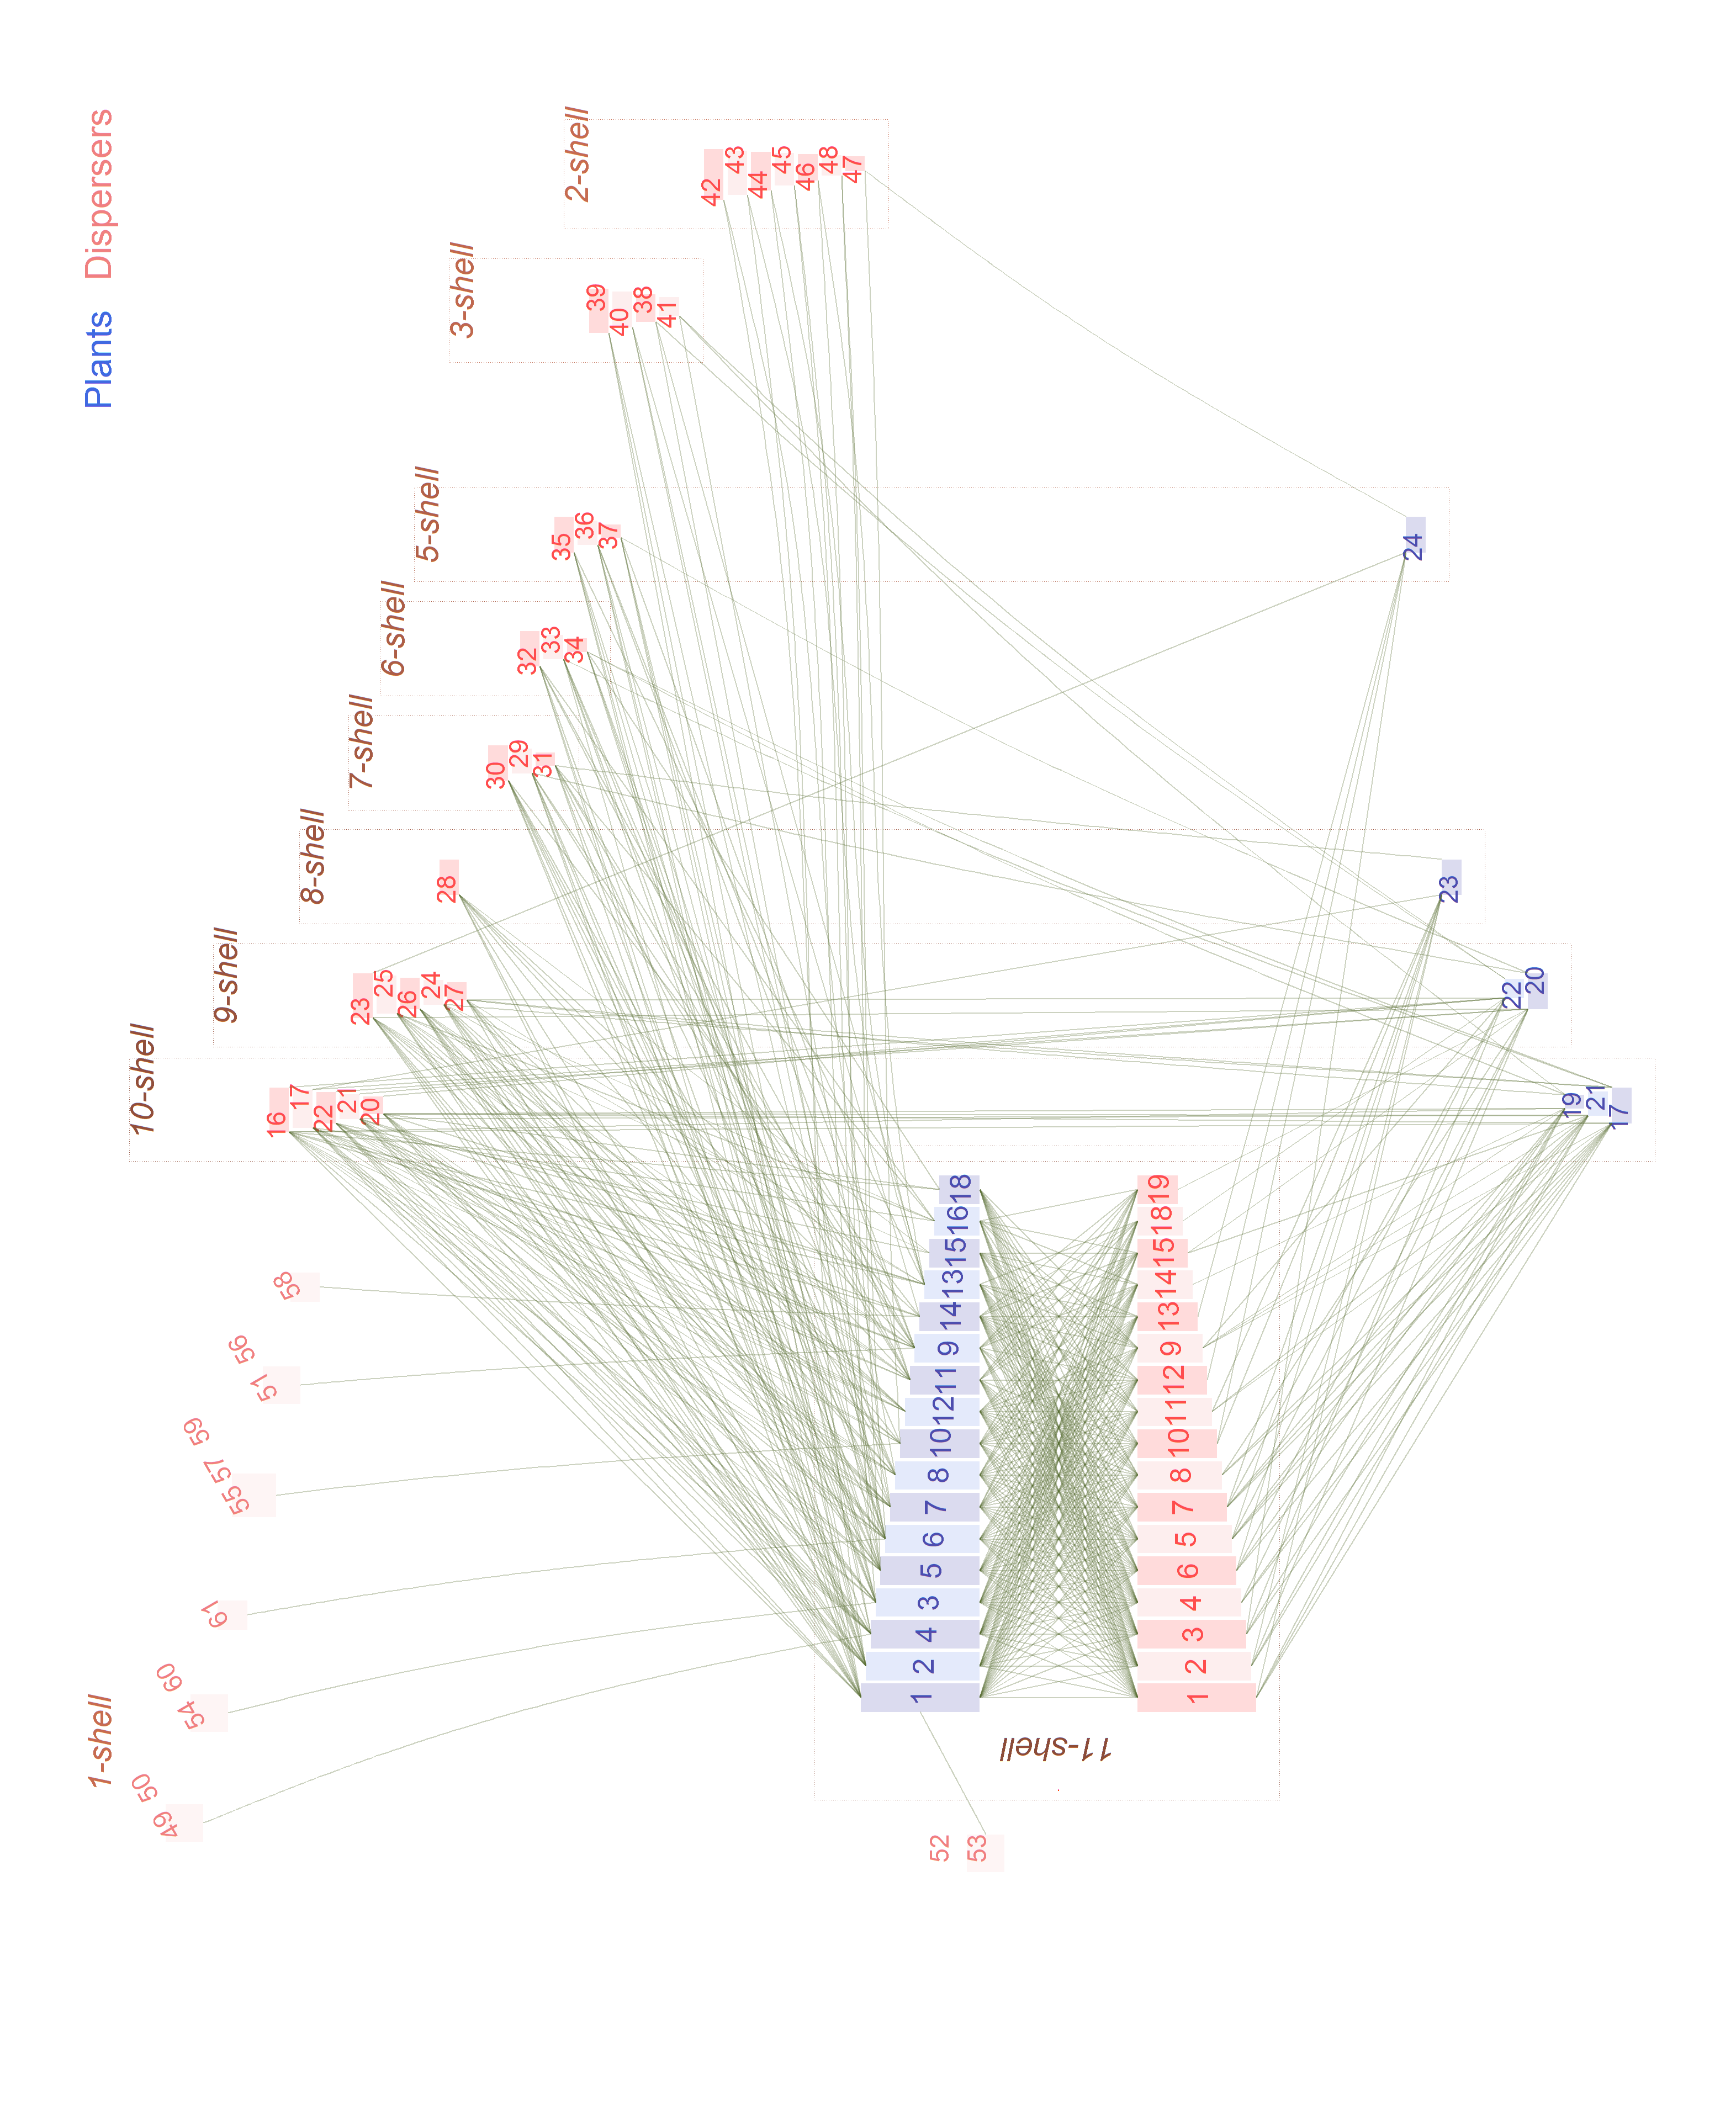
\includegraphics[scale=0.20]{Figures/VIS_M_SD_016_ziggurat.png}
\caption {Red de aves frugívoras $M\_SD\_016$ en la selva Kuala Lompat, Reserva de Krau Game, Malasia \cite{lambert1989fig}, con $85$ especies y $500$ enlaces.}
\label{fig:VIS_M_PL_047_ziggurat}
\end{figure}

\clearpage
\begin{figure}[ht!]
\centering
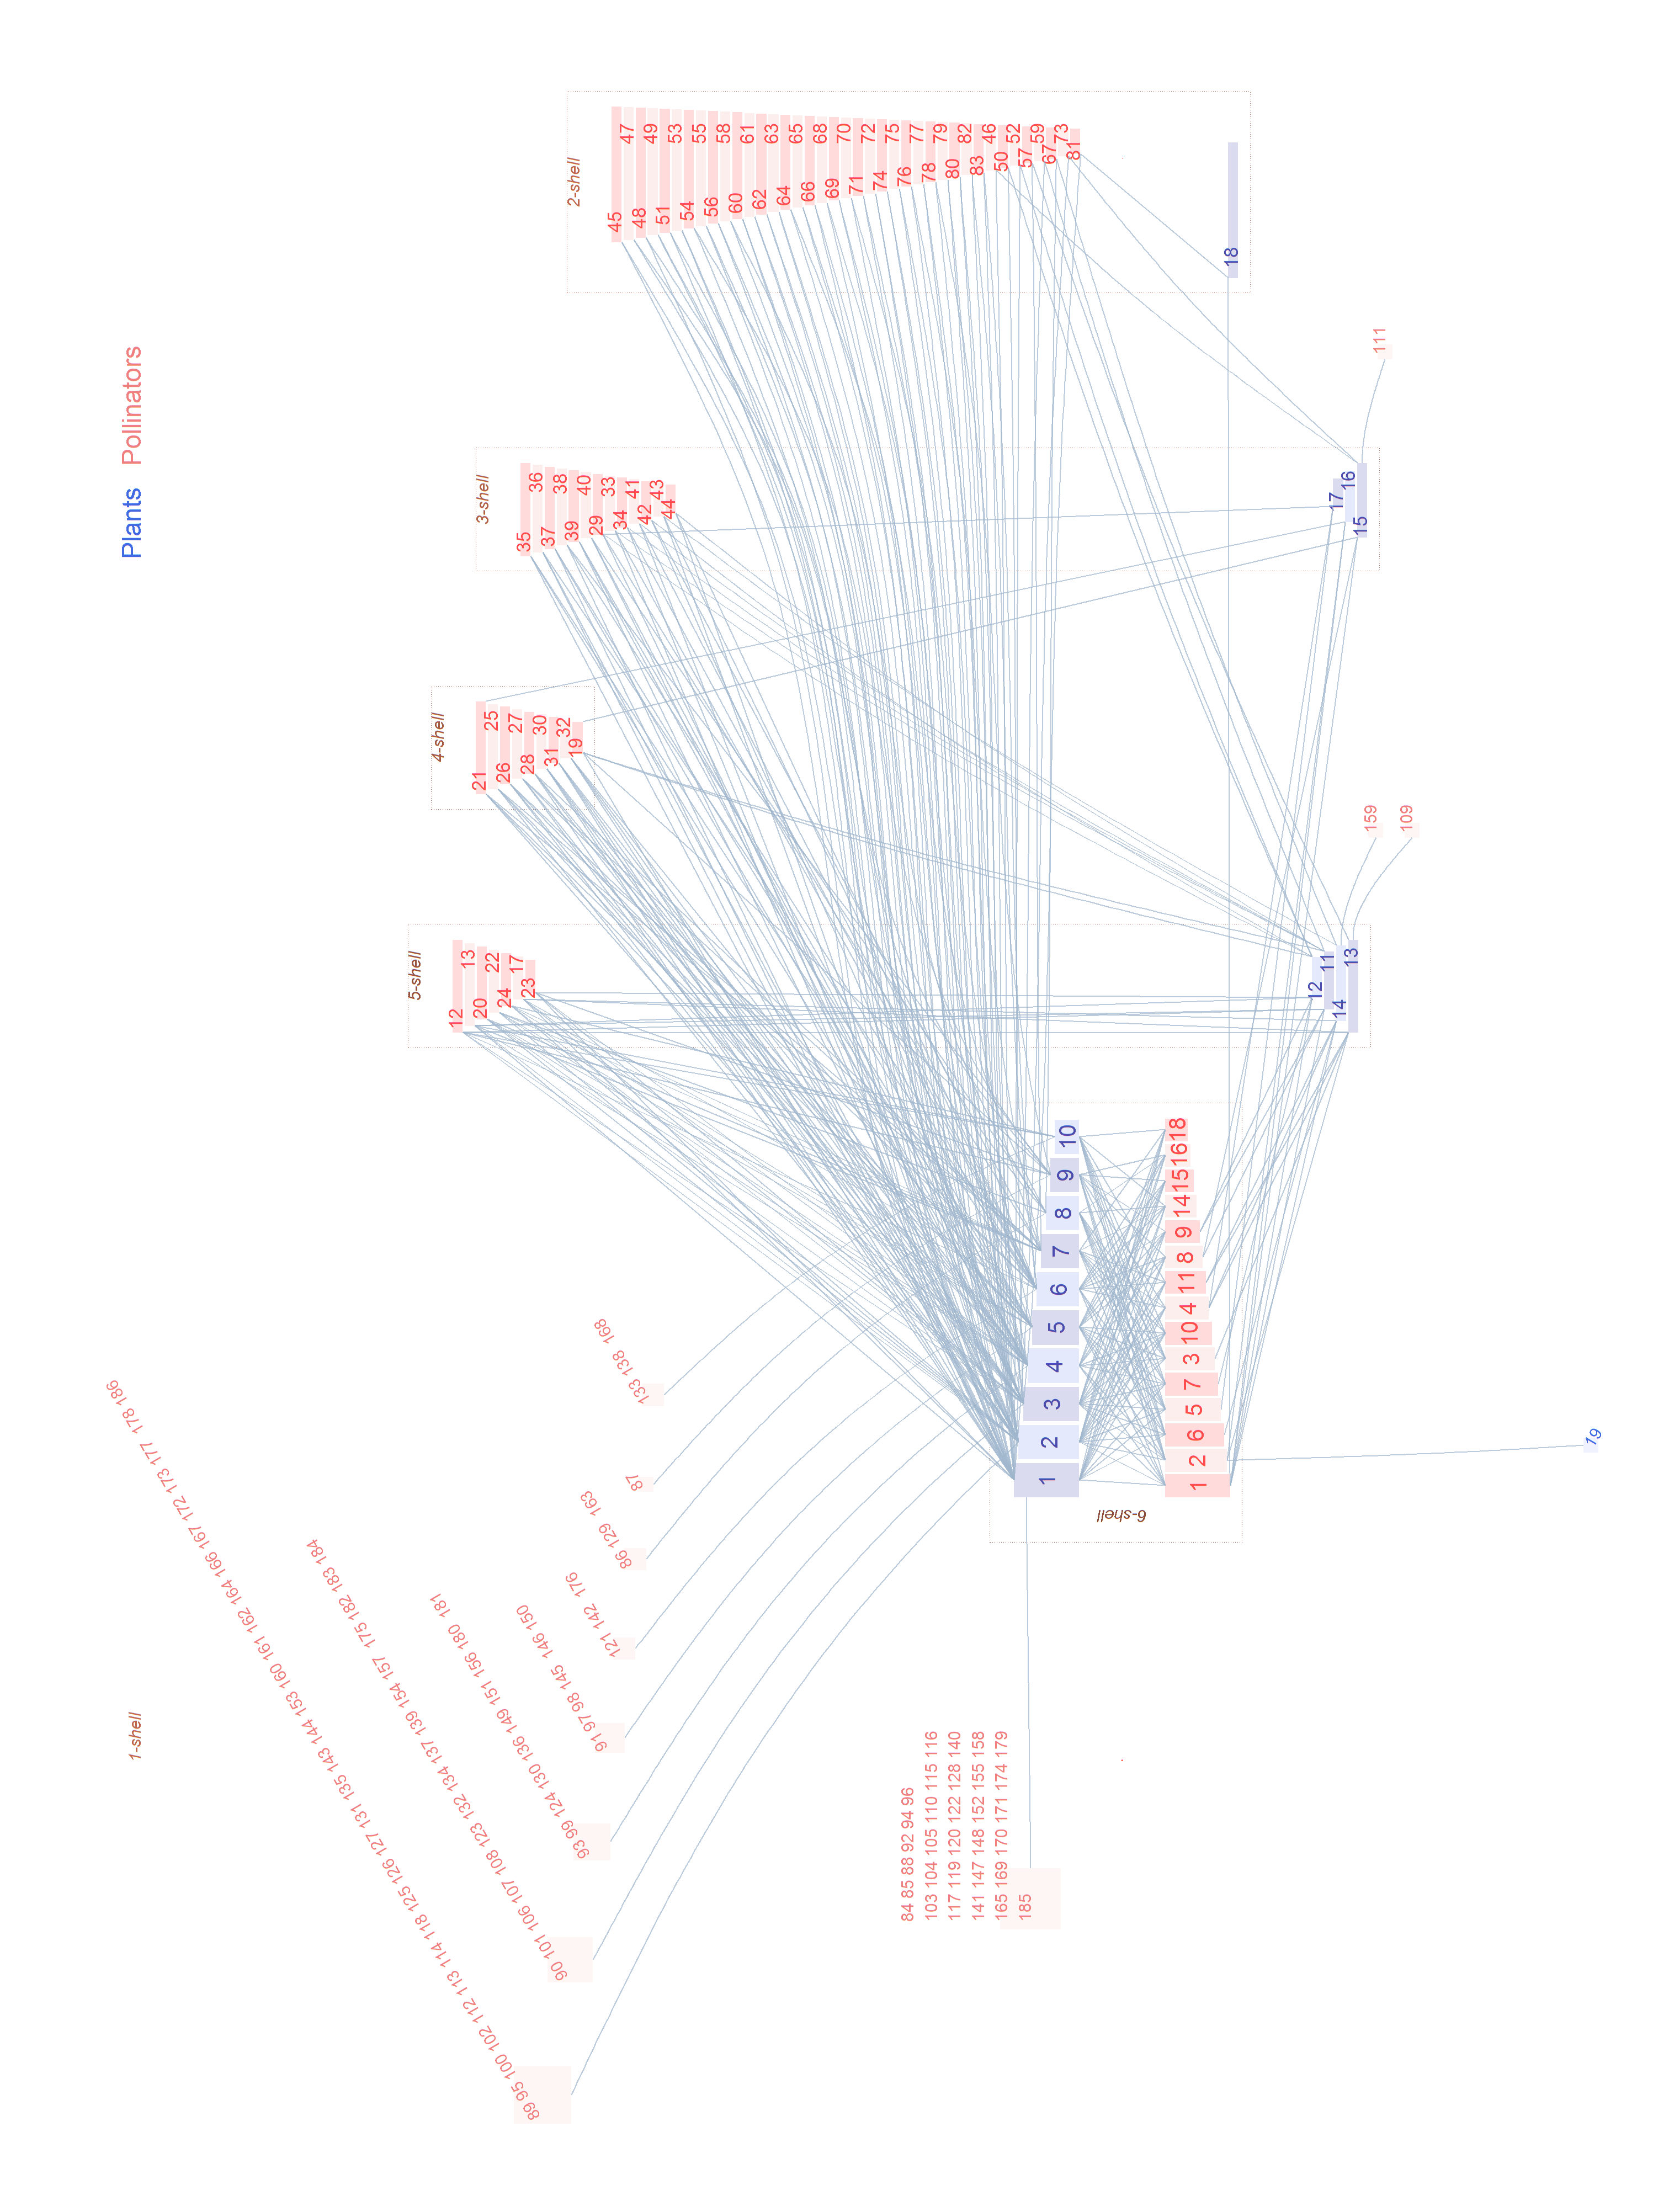
\includegraphics[scale=0.20]{Figures/VIS_M_PL_047_ziggurat.png}
\caption {Red de polinizadores $M\_PL\_047$, de un brezal en Isen Bjerg, Dinamarca \cite{dupont2009ecological}, con $205$ especies y $425$ enlaces.}
\label{fig:VIS_M_PL_047_ziggurat}
\end{figure}


\clearpage
\section{Resultados}

Nunc posuere quam at lectus tristique eu ultrices augue venenatis. Vestibulum ante ipsum primis in faucibus orci luctus et ultrices posuere cubilia Curae; Aliquam erat volutpat. Vivamus sodales tortor eget quam adipiscing in vulputate ante ullamcorper. Sed eros ante, lacinia et sollicitudin et, aliquam sit amet augue. In hac habitasse platea dictumst.


\section{Conclusiones}

Nunc posuere quam at lectus tristique eu ultrices augue venenatis. Vestibulum ante ipsum primis in faucibus orci luctus et ultrices posuere cubilia Curae; Aliquam erat volutpat. Vivamus sodales tortor eget quam adipiscing in vulputate ante ullamcorper. Sed eros ante, lacinia et sollicitudin et, aliquam sit amet augue. In hac habitasse platea dictumst.
